\documentclass[acmsmall,screen,review,anonymous]{acmart}

\usepackage{booktabs}
\usepackage{multirow}
\usepackage{amsmath}
\usepackage{amsthm}
\usepackage{graphicx}
\usepackage{xspace}
\usepackage{kotex}
\usepackage{flafter}
\usepackage{tikz}
\usetikzlibrary{arrows.meta,positioning}

\setcopyright{none}
\settopmatter{printacmref=true,printfolios=true}
\renewcommand\footnotetextcopyrightpermission[1]{}
\citestyle{acmauthoryear}

\acmConference[FSE '27]{ACM International Conference on the Foundations of Software Engineering}{July 12--16, 2027}{Shenzhen, China}
\acmYear{2027}
\acmMonth{7}
\copyrightyear{2027}
\acmDOI{}
\acmISBN{}


\title[Target Construction and Candidate Breadth in Program Repair]{Disentangling Candidate Breadth, Target Provenance, and Trajectory Supervision in Execution-Guided Program Repair}

\author{Anonymous Author(s)}
\affiliation{%
  \institution{Anonymous Institution}
  \country{Anonymous}
}

\begin{document}

\begin{abstract}
우리는 수리 목표(repair target) 구성과 실행 기반으로 선택되는 후보 폭(candidate breadth)을 분리하는 궤적 지도(trajectory supervision) 프레임워크인 \textsc{ZPDPatch}를 제시한다. 제출 이력은 중간 목표와 최종 목표를 제공하지만, 그 겉보기 이점은 추가 생성 기회와 교란될 수 있다. 997개의 Seen 입력과 문제 단위로 분리된(problem-held-out) 250개의 Python 입력에서, 출처와 개수를 일치시킨 학습은 커버리지--국소성(coverage--locality) 트레이드오프를 식별한다: 최종 Answer 목표는 중간 Progress 목표보다 수리율이 19.2/11.2 포인트 높은 반면, Progress 수리는 AST 편집 단위가 10.08/6.83만큼 더 작고 원본 토큰을 5.6/6.5 포인트 더 보존한다. 학생 단위로 분리된 Java 데이터에서의 직접 재학습은 이 트레이드오프를 재현한다: Answer는 85.6\%, Progress는 50.8\%를 수리하며, 공동 수리(joint repair)에서 Progress는 어휘 토큰을 4.8 포인트 더 보존한다. 결과와 거리가 일치하는 동료(peer) 목표는 Python Progress 커버리지를 추가로 4.3/6.0 포인트 높인다. 이와 별개로, 디코더를 고정한 1회 대 3회 추출(draw) 비교는 Seen에서 15.1 포인트를 산출한다. 현재 코드만 사용하는(current-only) 4셀 비교는 반복 확률적 추출을 넘어서는 체크포인트 정체성(checkpoint identity)의 강건한 추가 이득을 발견하지 못하며, 추론 스택(inference stack)에 대한 민감성을 드러낸다. 우리의 컨트롤러는 관측된 테스트에 대한 비퇴행(non-regression)과 선택적인 유한 편집 예산 준수를 보장한다. 검증된 Transformers current-only Answer 3개 조합은 72.0/81.2\%를 수리하지만, 편집 제한이 없을 때 Seen에서는 검색 기반 LSGen이 여전히 더 강하다. 이러한 통제 실험들은 목표 구성을 후보 폭과 구별되는 수리 국소성 메커니즘으로 식별하며, 교육적 이점은 주장하지 않는다.
% We present \textsc{ZPDPatch}, a trajectory-supervision framework that separates repair-target construction from execution-selected candidate breadth. Submission histories provide intermediate and terminal targets, but their apparent benefit can be confounded by extra generation opportunities. On 997 Seen and 250 problem-held-out Python inputs, source- and count-matched training identifies a coverage--locality tradeoff: terminal Answer targets gain 19.2/11.2 repair-rate points over intermediate Progress targets, whereas Progress repairs are 10.08/6.83 AST-edit units smaller and retain 5.6/6.5 more source-token points. Direct retraining on student-disjoint Java data replicates the tradeoff: Answer repairs 85.6\% versus 50.8\%, while Progress retains 4.8 more lexical-token points on joint repairs. Outcome- and distance-matched peer targets further raise Python Progress coverage by 4.3/6.0 points. Separately, a fixed-decoder one-to-three-draw contrast yields 15.1 Seen points. A current-only four-cell comparison finds no robust additional checkpoint-identity gain over repeated stochastic draws and exposes inference-stack sensitivity. Our controller guarantees observed-test non-regression and optional finite edit-budget compliance. The tested Transformers current-only Answer triple repairs 72.0/81.2\%, although retrieval-based LSGen remains stronger on Seen without an edit limit. These controls identify target construction as a repair-locality mechanism, distinct from candidate breadth and without claiming educational benefit.
\end{abstract}

\ccsdesc[500]{Software and its engineering~Software testing and debugging}
\ccsdesc[300]{Applied computing~Education}
\ccsdesc[300]{Computing methodologies~Natural language generation}

\keywords{automated program repair, programming education, large language models, submission trajectories, execution-guided repair}

\maketitle

\section{Introduction}
\label{sec:introduction}

온라인 저지(online judge)는 반복적인 프로그램 수정 이력을 대규모로 기록하지만, 조악한 판정(verdict)만으로는 어떤 편집이 실행 가능한 해답을 향해 진전하는지 설명하지 못한다. 우리는 이러한 제출 시퀀스를 수리 지도 신호로 사용한다.
% Online judges record iterative program revisions at scale, but coarse verdicts do not explain which edits progress toward a viable solution. We use these submission sequences as repair supervision.

자동 프로그램 수리(APR)는 실행 가능하고 코드에 특화된 피드백을 제공한다. 이 분야는 탐색 기반 생성-검증(generate-and-validate) 수리, 학습된 변환, 테스트 기반 검증을 아우른다~\cite{weimer2009automatically,legoues2012genprog,gazzola2019automatic,monperrus2018automatic}. 프로그래밍 과제를 위한 시스템들은 동료 해답을 군집화하거나, 사용자의 코드를 참조 해답에 정렬하거나, 수정된 프로그램을 합성한다~\cite{gulwani2018automated,wang2018search,hu2020re}. 보다 최근의 시스템들은 언어 모델, 실행 진단, 검색된 예제, 반복적 대화를 사용한다~\cite{joshi2023repair,zhang2024pydex,yang2024cref,liu2024fastfixer,orvalho2025counterexample}. 대부분은 최신 버그 프로그램을 조건으로 하며 경우에 따라 테스트나 동료 프로그램으로 보강하지만, 동일 사용자의 이전 제출물이 일급(first-class) 수리 문맥으로 쓰이는 경우는 드물다.
% Automated program repair (APR) offers executable, code-specific feedback. The field spans search-based generate-and-validate repair, learned transformations, and test-guided validation~\cite{weimer2009automatically,legoues2012genprog,gazzola2019automatic,monperrus2018automatic}. Systems for programming assignments cluster peer solutions, align a user's code to a reference, or synthesize a fixed program~\cite{gulwani2018automated,wang2018search,hu2020re}. More recent systems use language models, execution diagnostics, retrieved examples, and iterative conversations~\cite{joshi2023repair,zhang2024pydex,yang2024cref,liu2024fastfixer,orvalho2025counterexample}. Most condition on the latest buggy program, possibly augmented with tests or peer programs; earlier submissions by the same user are rarely first-class repair context.

두 사용자는 서로 다른 수정 시도를 거쳐 유사한 코드에 도달할 수 있다. 교육적 관점에서, 입증된 개선은 근접 발달 영역(Zone of Proximal Development, ZPD)과 닮아 있다~\cite{cole1978mind,murray2002toward,chounta2017grey}. 우리는 이러한 궤적이 수리 지도를 개선하는지 검증한다. ZPD는 이 설계의 동기가 되지만, 측정된 심리학적 구성 개념이나 학습 성과는 아니다.
% Two users can reach similar code through different attempted revisions. In educational terms, demonstrated improvements resemble the Zone of Proximal Development (ZPD)~\cite{cole1978mind,murray2002toward,chounta2017grey}. We test whether those trajectories improve repair supervision. ZPD motivates this design but is not a measured psychological construct or learning outcome.

그림~\ref{fig:overview}는 \textsc{ZPDPatch}를 보여준다. \textsc{Progress}는 판정 개선과 동일 판정 내의 테스트별 개선을 채굴하고, \textsc{Strict}는 더 나은 판정을 요구하며, \textsc{Answer}는 각 실패를 최종 정답(acceptance)과 짝짓는다. 관계(relation)마다 세 개의 QLoRA 시드를 사용하여 아홉 개의 체크포인트를 만든다. 검증으로 세 개를 선택하고, 선택적인 AST 트리 편집 거리(TED)를 동반한 실행이 수용과 기권(abstention)을 제어한다.
% Figure~\ref{fig:overview} presents \textsc{ZPDPatch}. \textsc{Progress} mines verdict improvements and same-verdict per-test improvements; \textsc{Strict} requires a better verdict; \textsc{Answer} pairs each failure with final acceptance. Three QLoRA seeds per relation produce nine checkpoints. Validation selects three, and execution with optional AST tree edit distance (TED) controls acceptance and abstention.

우리의 주된 기여는 혼동하기 쉬운 메커니즘들, 즉 출력 샘플링, 독립적인 학습 시드, 검증으로 선택된 풀(pool) 폭, 관계별 데이터셋 구성, 목표 출처(provenance), 이전 제출물의 직렬화에 대한 실증적 식별 및 보고 설계이다. \(A_1\!\rightarrow T_1\!\rightarrow S_3\!\rightarrow A_3\!\rightarrow A_9\!\rightarrow M_9\) 사다리는 연속된 각 기회를 일치시킨다. 목표를 일치시킨 재학습에서는 이전 제출물 직렬화의 안정적인 인과적 이점이 발견되지 않는 반면, 짝지은 목표(paired-target) 학습은 재현 가능한 트레이드오프를 식별한다: 최종 Answer 목표는 커버리지를 높이고, 중간 Progress 목표는 더 작고 원본을 더 많이 보존하는 수리를 만든다.
% Our primary contribution is an empirical identification and reporting design for mechanisms that are easy to conflate: output sampling, independent training seeds, validation-selected pool breadth, relation-specific dataset construction, target provenance, and serialization of prior submissions. The \(A_1\!\rightarrow T_1\!\rightarrow S_3\!\rightarrow A_3\!\rightarrow A_9\!\rightarrow M_9\) ladder matches each successive opportunity. Target-matched retraining finds no stable causal benefit from serializing earlier submissions, while paired-target training identifies a reproducible tradeoff: terminal Answer targets raise coverage, whereas intermediate Progress targets produce smaller, more source-preserving repairs.

본 논문의 기여는 다음과 같다:
% This paper makes the following contributions:
\begin{itemize}
  \item 우리는 여덟 편의 교육용 수리 연구에 대한 범위를 한정한 감사(audit)를 통해 후보 폭을 충분히 보고되지 않은 교란 요인으로 식별하고, 동일 추출(same-draw) 분해를 도출하며, 1회 추출 품질, 실행 기반으로 선택된 커버리지, 배포 시 호출 수를 분리하는 보고 규약을 명시한다.
  % \item We identify candidate breadth as an underreported confound through a scoped audit of eight educational repair studies, derive a same-draw decomposition, and specify a reporting contract separating one-draw quality, execution-selected coverage, and deployed calls.
  \item 우리는 세 가지 유한한 실행 증거 관계를 구성하고, 체크포인트 선택을 정확한 검증 커버리지 탐색으로 풀며, 비퇴행, 후보 상대적 완전성, 편집 예산 준수를 위한 생성기 독립적(generator-agnostic) 컨트롤러 규약을 제공하는 궤적 지도 프레임워크를 제시한다.
  % \item We present a trajectory-supervision framework that constructs three finite execution-evidence relations, solves checkpoint choice as exact validation-coverage search, and provides a generator-agnostic controller contract for non-regression, candidate-relative completeness, and edit-budget compliance.
  \item 우리는 이력, 목표, 목표 출처를 일치시킨 통제, 5겹 문제 교차적합(cross-fitted) 선택, 숨겨진 테스트, 두 가지 모델 규모, 두 개의 Java 홀드아웃, 패치 국소성 분석으로 전체 \(A_1\)--\(T_1\)--\(S_3\)--\(A_3\)--\(A_9\)--\(M_9\) 메커니즘 사다리를 평가한다. 이 증거는 고정 디코더 폭 이득, 일치된 동료 선택으로 인한 커버리지 이득, 그리고 Python과 학생 분리 Java에서 직접 재현된 목표 커버리지/국소성 트레이드오프를 구별한다.
  % \item We evaluate the full \(A_1\)--\(T_1\)--\(S_3\)--\(A_3\)--\(A_9\)--\(M_9\) mechanism ladder with matched history, target, and target-provenance controls, five-fold problem-cross-fitted selection, hidden tests, two model scales, two Java holdouts, and patch-locality analyses; the evidence distinguishes fixed-decoder breadth gains, coverage gains from matched peer selection, and a directly replicated target-coverage/locality tradeoff on Python and student-disjoint Java.
\end{itemize}

\section{Background and Related Work}
\label{sec:related}

\subsection{Structure- and Reference-Based Educational Repair}

교육용 APR은 하나의 명세에 대해 작성된 다수의 프로그램을 활용할 수 있다. CLARA는 수리를 추출하기 전에 프로그램을 군집화하고 정렬하며, SARFGEN은 참조 프로그램을 탐색하고 정렬하고, Refactory는 비교 전에 리팩터링을 정규화한다~\cite{gulwani2018automated,wang2018search,hu2020re}. 임베딩, 해답 공간 모델, 시각화는 주석을 전파하거나 반복되는 전략을 드러내며, 다중 함수 및 다양화 방법은 목표를 단일 수정 이상으로 넓힌다~\cite{piech2015embeddings,glassman2015overcode,rivers2017datadriven,yi2017feasibility,heo2023referent,choi2021automated,choi2025automated}.
% Educational APR can exploit many programs written for one specification. CLARA clusters and aligns programs before extracting a repair; SARFGEN searches and aligns reference programs; Refactory normalizes refactorings before comparison~\cite{gulwani2018automated,wang2018search,hu2020re}. Embeddings, solution-space models, and visualization propagate annotations or expose recurring strategies, while multi-function and diversified methods broaden the target beyond one correction~\cite{piech2015embeddings,glassman2015overcode,rivers2017datadriven,yi2017feasibility,heo2023referent,choi2021automated,choi2025automated}.

LSGen은 편집 정보를 사용하여 과거 수리 쌍을 검색하고, 생성하며, 다시 검색할 수 있다~\cite{dai2026learner}. LSGen은 대상 문제에 대한 다른 사용자들의 Seen-Train 해답을 보유하는데, 이는 완전히 새로운 과제에서는 사용할 수 없으므로, 사용할 수 없는 참조를 제공하는 대신 Unseen에서 LSGen을 제외한다.
% LSGen retrieves historical repair pairs using edit information, generates, and may retrieve again~\cite{dai2026learner}. It retains other users' Seen-Train solutions for the target problem; these are unavailable for genuinely new assignments, so we exclude LSGen from Unseen rather than supply unavailable references.

\subsection{Neural and Large-Language-Model Repair}

생성-검증 APR은 광범위한 탐색의 이점과 테스트 과적합 위험을 드러낸다~\cite{weimer2009automatically,legoues2012genprog,qi2014strength,smith2015cure}. 신경망 수리는 저장소 변환이나 문맥 인식 번역을 학습하며~\cite{tufano2019empirical,lutellier2020coconut,yasunaga2021break,xia2022less,jiang2023impact}, RING, PyDex, FastFixer는 교육을 위해 조건부 생성을 특화한다~\cite{joshi2023repair,zhang2024pydex,zhang2022repairing,liu2024fastfixer}. 동료 검색과 구문 위치 식별은 후보를 제약하지만~\cite{zhao2024peer,phung2023generating}, 여전히 실행 검증이 필요하다.
% Generate-and-validate APR exposes broad-search benefits and test-overfitting risks~\cite{weimer2009automatically,legoues2012genprog,qi2014strength,smith2015cure}. Neural repair learns repository transformations or context-aware translation~\cite{tufano2019empirical,lutellier2020coconut,yasunaga2021break,xia2022less,jiang2023impact}; RING, PyDex, and FastFixer specialize conditional generation for education~\cite{joshi2023repair,zhang2024pydex,zhang2022repairing,liu2024fastfixer}. Peer retrieval and syntax localization constrain candidates~\cite{zhao2024peer,phung2023generating}, but still require execution validation.

실행 인식(execution-aware) 방법은 모델 신뢰도와 독립적인 신호로 이러한 우려를 다룬다. SelfAPR은 테스트 진단으로부터 학습하고, FixEval은 실행을 수리 평가 기준으로 삼으며, CREF는 수리 대화 전반에 진단을 전달하고, 반례 기반 수리는 생성, 결함 위치 식별, MaxSAT를 결합한다~\cite{ye2022selfapr,haque2023fixeval,yang2024cref,orvalho2025counterexample}. \textsc{ZPDPatch} 역시 후보를 실행하지만, 다른 단위의 지도와 제어를 도입한다. 실제(authentic) 궤적은 합성된 오염이나 수동으로 지정된 수리 역할 대신 실행 증거 개선 관계를 정의한다. 구성원들은 기반 모델을 공유하여 상관된 오류를 가질 수 있지만, 생성은 비적응적이다: 어떤 구성원도 다른 구성원의 출력을 입력으로 받지 않는다. 변경되지 않은 프로그램은 항상 선택 가능하므로, 생성 실패가 퇴행을 강제할 수 없다.
% Execution-aware methods address those concerns with signals independent of model confidence. SelfAPR learns from test diagnostics; FixEval makes execution the repair-evaluation criterion; CREF carries diagnostics through a repair conversation; counterexample-guided repair combines generation, fault localization, and MaxSAT~\cite{ye2022selfapr,haque2023fixeval,yang2024cref,orvalho2025counterexample}. \textsc{ZPDPatch} likewise executes candidates, but introduces a different unit of supervision and control. Authentic trajectories define execution-evidence improvement relations rather than synthetic corruptions or manually assigned repair roles. Members share a base model and may have correlated errors, but generation is non-adaptive: no member consumes another member's output. The unchanged program remains selectable, so a failed generation cannot force a regression.

\subsection{Adaptive Feedback, ZPD, and Submission Histories}

피드백 연구는 정답 여부를 넘어서는 실행 가능한(actionable) 정보를 강조한다~\cite{keuning2018systematic,narciss2008feedback,hattie2007power,shute2008focus}. 튜터링, iSnap, LLM 힌트는 도움 요청과 다음 단계의 세분성을 다룬다~\cite{aleven2000limitations,price2017isnap,roest2024next,xiao2024exploring,heickal2024generating}. ZPD는 독립적 수행과 조력 수행 사이의 지원에 동기를 부여한다~\cite{cole1978mind,murray2002toward,chounta2017grey,schulze2024beyond}. 우리가 관측한 도달 가능성은 이보다 좁으며, 학습이나 최적의 스캐폴딩을 입증하지 않는다.
% Feedback research emphasizes actionable information beyond correctness~\cite{keuning2018systematic,narciss2008feedback,hattie2007power,shute2008focus}. Tutoring, iSnap, and LLM hints address help seeking and next-step granularity~\cite{aleven2000limitations,price2017isnap,roest2024next,xiao2024exploring,heickal2024generating}. ZPD motivates support between independent and assisted performance~\cite{cole1978mind,murray2002toward,chounta2017grey,schulze2024beyond}; our observed reachability is narrower and does not establish learning or optimal scaffolding.

지식 추적(knowledge tracing)은 상호작용 이력으로부터 잠재적 숙달도를 추정한다~\cite{corbett1994knowledge,piech2015deep,ghosh2020context}. 반면 \textsc{ZPDPatch}는 숙달도를 추론하거나 학습을 예측하지 않고, 실행 증거에 따라 코드 상태를 정렬한다.
% Knowledge tracing estimates latent mastery from interaction histories~\cite{corbett1994knowledge,piech2015deep,ghosh2020context}. \textsc{ZPDPatch} instead orders code states by execution evidence, without inferring mastery or predicting learning.

\subsection{Positioning of This Work}

참조 정렬 방식 및 LSGen과 달리, \textsc{ZPDPatch}는 동일 문제의 해답 저장소를 필요로 하지 않는다. 딥 앙상블이나 모델 수프와 달리, 확률이나 가중치를 집계하는 대신 완전한 프로그램을 실행한다~\cite{lakshminarayanan2017simple,wortsman2022model}. 동일 목표 Answer 풀은 혼합 목표 풀의 체크포인트 수, 검증 탐색, 생성 예산을 일치시켜, 관계 지도가 시드 다양성 이상의 무언가를 더하는지 검증한다.
% Unlike reference alignment and LSGen, \textsc{ZPDPatch} needs no same-problem solution repository. Unlike deep ensembles or model soups, it executes complete programs rather than aggregating probabilities or weights~\cite{lakshminarayanan2017simple,wortsman2022model}. A same-target Answer pool matches the mixed-target pool's checkpoint count, validation search, and generation budget, testing whether relation supervision adds more than seed diversity.

반복 샘플링은 코드 분야에서 확립된 추론 스케일링 메커니즘이다: 독립적인 추출들이 서로 다른 성공 프로그램을 포괄할 때 pass@$k$가 상승한다~\cite{chen2021evaluating}. 우리는 이 효과를 새로운 것으로 주장하지 않는다. 대신, 우리의 동일 추출 \(T_1\)--\(S_3\) 구성은 APR 컨트롤러 내부에서 그 정확한 기여도를 측정한 뒤, 3회 호출 예산을 고정한 채 독립 체크포인트나 관계 채굴 목표가 샘플링만으로 얻는 것 이상의 커버리지나 구조적 국소성을 더하는지 검증한다.
% Repeated sampling is an established inference-scaling mechanism for code: pass@$k$ rises when independent draws cover different successful programs~\cite{chen2021evaluating}. We do not claim that effect as novel. Instead, our same-draw \(T_1\)--\(S_3\) construction measures its exact contribution inside an APR controller, then holds the three-call budget fixed while testing whether independent checkpoints or relation-mined targets add coverage or structural locality beyond sampling alone.

\paragraph{A scoped audit of candidate accounting.}
표~\ref{tab:breadth-audit}는 확장된 폭 결과 이전에 고정된 규칙을 사용하여, 직접 관련된 신경망 또는 LLM 기반 교육용 수리 연구 여덟 편을 코딩한다. 다섯 편은 다수의 생성 기회를 배포하거나 주로 평가한다. EPR 벤치마크만이 pass@1/5/10을 보고하고, CREF는 TOP-5 옆에 AVG-5를 제시하며, PyDex, 반례 기반 수리, LSGen은 일치된 단일 후보 통제로 추가 기회를 분리하지 않는다~\cite{zhang2024pydex,koutcheme2024benchmarking,yang2024cref,orvalho2025counterexample,dai2026learner}. 적응적 반복은 새로운 증거를 가져올 수 있으므로, 이 관찰은 해당 방법들을 무효화하기보다 명시적인 후보 계정(accounting)의 필요성을 뒷받침한다.
% Table~\ref{tab:breadth-audit} codes eight directly related neural or LLM educational-repair studies using a rule frozen before our extended breadth results. Five deploy or primarily evaluate multiple generated opportunities. Only the EPR benchmark reports pass@1/5/10, while CREF exposes AVG-5 beside TOP-5; PyDex, counterexample-guided repair, and LSGen do not isolate extra opportunities with a matched one-candidate control~\cite{zhang2024pydex,koutcheme2024benchmarking,yang2024cref,orvalho2025counterexample,dai2026learner}. Adaptive iterations can carry new evidence, so this observation motivates explicit candidate accounting rather than invalidating those methods.

\begin{table}[tbp]
\caption{후보 계정에 대한 범위 한정 감사. ``1-draw''는 다중 기회 커버리지에 일치된 단일 기회 수치가 함께 제시되는지를 묻고, ``partial''은 TOP-5 옆에 AVG-5가 제시됨을 뜻한다. 아티팩트에 출처와 NR 필드가 기록되어 있다.}
% \caption{Scoped audit of candidate accounting. ``1-draw'' asks whether a
% matched single-opportunity quantity accompanies multi-opportunity coverage;
% ``partial'' denotes AVG-5 beside TOP-5. The artifact records sources and NR
% fields.}
\label{tab:breadth-audit}
\centering
\scriptsize
\setlength{\tabcolsep}{3pt}
\begin{tabular}{lccc}
\toprule
Study & Opportunities & Union/iterate & 1-draw \\
\midrule
PyDex/MMAPR~\cite{zhang2024pydex,zhang2022repairing} & 10/phase & yes & no \\
EPR benchmark~\cite{koutcheme2024benchmarking} & 1/5/10 & yes & yes \\
CREF~\cite{yang2024cref} & 5 & yes & partial \\
PaR~\cite{zhao2024peer} & NR + oracle & oracle & no \\
FastFixer~\cite{liu2024fastfixer} & 1 reported & no & n/a \\
CEGIS repair~\cite{orvalho2025counterexample} & 1--7 & yes & no \\
LSGen~\cite{dai2026learner} & 3 & yes & no \\
REFERENT~\cite{heo2023referent} & NR & NR & NR \\
\bottomrule
\end{tabular}
\end{table}

이 목적 표집(purposive) 감사는 여덟 편의 연구만을 다룬다. 이 보고 규약은 동일 디코더 1회 추출 RR, 배포된 각 $k$에서의 합집합 커버리지, 고정된 선택 규칙, 명시적 시간 단위를 갖는 호출 수를 요구한다. RQ4가 이러한 수치를 제공한다. 우리의 비적응적 후보는 정확한 재연(replay)을 허용하지만, 적응적 피드백 방법은 후보 분포를 바꿀 수 있어 다른 계정 방식이 필요하다.
% This purposive audit covers only eight studies. Its reporting contract requires same-decoder one-draw RR, union coverage at each deployed $k$, a fixed selection rule, and calls with explicit timing units. RQ4 supplies these quantities. Our non-adaptive candidates permit exact replay; adaptive feedback methods can change the candidate distribution and require different accounting.

\section{Problem Formulation}
\label{sec:formulation}

문제 \(p\)에 대해 사용자의 \(i\)번째 제출을 \(s_i=(c_i,v_i)\)라 하자. 여기서 \(c_i\)는 완전한 소스 코드이고 \(v_i\)는 온라인 저지 판정이다. 제출 궤적 \(\tau=[s_1,s_2,\ldots,s_n]\)은 시간순으로 정렬되며 첫 번째 정답(accepted) 제출에서 끝난다. \(d_p\)는 문제 설명과 자원 제약을 포함하고, \(\mathcal{E}_p\)는 사용 가능한 테스트 스위트라 하자. \(c_i\)를 재실행하면 테스트별 결과 벡터 \(o_i=(o_i(e))_{e\in\mathcal{E}_p}\)를 얻는다.
% For problem \(p\), let a user's \(i\)-th submission be \(s_i=(c_i,v_i)\), where \(c_i\) is the complete source code and \(v_i\) is the online-judge verdict. A submission trajectory \(\tau=[s_1,s_2,\ldots,s_n]\) is chronologically ordered and terminates at the first accepted submission. Let \(d_p\) contain the problem statement and resource constraints, and let \(\mathcal{E}_p\) be the available test suite. Re-executing \(c_i\) gives a per-test outcome vector \(o_i=(o_i(e))_{e\in\mathcal{E}_p}\).

수리 예제는 문제 문맥 \(d_p\), 관측된 시퀀스 \(h\), 완전한 목표 프로그램 \(y\)로 구성된다. 어댑터별 규칙이 어떤 제출이 \(h\)에 남고 어떤 이후 제출이 \(y\)를 제공할지 결정하며, 두 제출이 원래 궤적에서 인접할 필요는 없다. \(x=(d_p,h)\)가 주어지면, 모델은 하나의 완전한 프로그램 \(\hat c\)를 생성한다.
% A repair example consists of problem context \(d_p\), an observed sequence \(h\), and a complete target program \(y\). Adapter-specific rules decide which submissions remain in \(h\) and which later submission supplies \(y\); the two need not be adjacent in the original trajectory. Given \(x=(d_p,h)\), a model generates one complete program \(\hat c\).

이후 상태가 같은 사용자의 궤적에 나타나고 어댑터별 개선 규칙을 만족하면, 그 상태를 \emph{도달 가능(reachable)}하다고 한다. 이 경험적 속성은 최소성이나 교육적 가치를 함의하지 않으며, 우리는 이런 방식으로 채굴된 목표가 현재 프로그램을 더 많이 보존하는지 검증한다.
% A later state is \emph{reachable} when it occurs in the same user's trajectory and satisfies an adapter-specific improvement rule. This empirical property does not imply minimality or educational value; we test whether targets mined this way preserve more of the current program.

\section{Approach}
\label{sec:approach}

\begin{figure}[t]
  \centering
  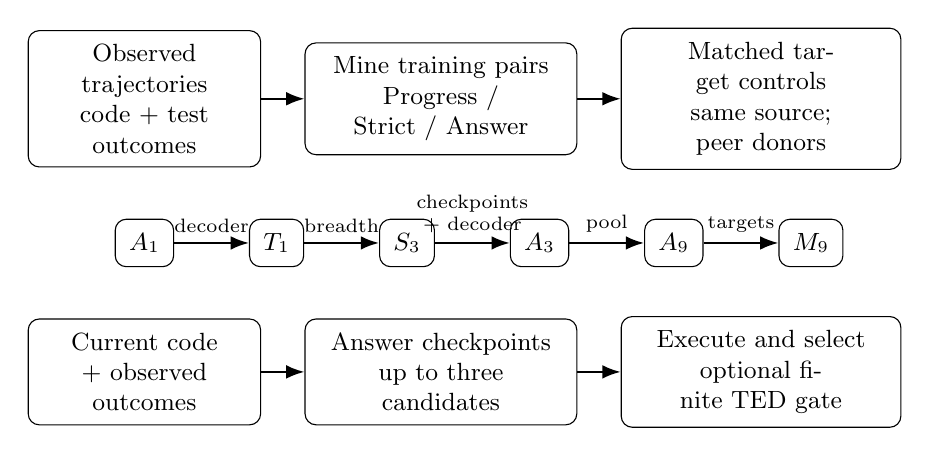
\begin{tikzpicture}[font=\small,box/.style={draw,rounded corners,align=center,inner sep=5pt},arr/.style={-{Latex},thick}]
    \node[box,text width=2.6cm] (history) {Observed trajectories\\code + test outcomes};
    \node[box,text width=3.1cm,right=0.55cm of history] (targets) {Mine training pairs\\Progress / Strict / Answer};
    \node[box,text width=3.2cm,right=0.55cm of targets] (match) {Matched target controls\\same source; peer donors};
    \draw[arr] (history)--(targets);
    \draw[arr] (targets)--(match);
    \node[below=0.65cm of history,box] (a1) {$A_1$};
    \node[right=0.95cm of a1,box] (t1) {$T_1$};
    \node[right=0.95cm of t1,box] (s3) {$S_3$};
    \node[right=0.95cm of s3,box] (a3) {$A_3$};
    \node[right=0.95cm of a3,box] (a9) {$A_9$};
    \node[right=0.95cm of a9,box] (m9) {$M_9$};
    \draw[arr] (a1)--node[above,font=\scriptsize]{decoder}(t1);
    \draw[arr] (t1)--node[above,font=\scriptsize]{breadth}(s3);
    \draw[arr] (s3)--node[above,font=\scriptsize,align=center]{checkpoints\\+ decoder}(a3);
    \draw[arr] (a3)--node[above,font=\scriptsize]{pool}(a9);
    \draw[arr] (a9)--node[above,font=\scriptsize]{targets}(m9);
    \node[box,text width=2.6cm,below=0.65cm of a1] (current) {Current code\\+ observed outcomes};
    \node[box,text width=3.1cm,right=0.55cm of current] (generate) {Answer checkpoints\\up to three candidates};
    \node[box,text width=3.2cm,right=0.55cm of generate] (return) {Execute and select\\optional finite TED gate};
    \draw[arr] (current)--(generate);
    \draw[arr] (generate)--(return);
  \end{tikzpicture}
  \caption{최종 식별 및 배포 설계. 이력으로부터 관계별 SFT 쌍을 오프라인에서 채굴한다. 일치된 $A_1\!\rightarrow T_1\!\rightarrow S_3\!\rightarrow A_3\!\rightarrow A_9\!\rightarrow M_9$ 사다리는 후보 폭, 체크포인트 효과, 풀 선택, 관계 목표를 분리한다. Transformers current-only $A_3$는 최대 세 개의 후보를 생성하며, 실행은 AC에서 멈추고 그렇지 않으면 비퇴행적이고 TED를 고려한 선택을 적용한다.}
  % \caption{Final identification and deployment design. Histories mine
  % relation-specific SFT pairs offline. The matched
  % $A_1\!\rightarrow T_1\!\rightarrow S_3\!\rightarrow A_3\!\rightarrow A_9\!\rightarrow M_9$
  % ladder separates candidate breadth, checkpoint effects, pool selection, and
  % relation targets. Transformers current-only $A_3$ generates up to three
  % candidates; execution stops on AC and otherwise applies non-regressive,
  % TED-aware selection.}
  \Description{Three rows show trajectory-derived target construction and matched-target controls; the A1-T1-S3-A3-A9-M9 mechanism ladder; and current-only A3 deployment with execution selection and an optional finite edit budget.}
  \label{fig:overview}
\end{figure}

\paragraph{Trajectory construction.}

우리는 제출을 문제와 사용자별로 묶고, 시간순으로 정렬한 뒤, 첫 정답에서 멈춘다. 들여쓰기/주석/빈 줄 정규화 후 연속된 중복만 제거하며, 연속되지 않은 재방문은 서로 다른 시도의 증거로 남긴다. 완전한 소스, 판정, 순서는 보존되며, 이력이나 전이(transition) 수의 최대값은 두지 않는다. 모든 상태는 재실행된다. 캐시 키는 문제, 정규화된 코드, 테스트 스위트 식별자, 시간 제한, 메모리 제한을 묶어 호환되지 않는 재사용을 방지한다. 러너 실패에는 명시적으로 가장 심각한 결과가 부여되며, Progress 구성은 완전한 캐시를 요구한다.
% We group submissions by problem and user, sort by time, and stop at first acceptance. After indentation/comment/blank-line normalization, we remove only consecutive duplicates; non-consecutive revisits remain evidence of distinct attempts. Complete source, verdict, and order are preserved, with no maximum history or transition count. Every state is re-executed. Cache keys bind problem, normalized code, test-suite identity, timeout, and memory limit, preventing incompatible reuse. Runner failures receive an explicit most-severe outcome, and Progress construction requires a complete cache.

\paragraph{Adapter-specific supervision.}
\label{sec:supervision}

우리는 \texttt{AC}에 심각도 0, \texttt{WA}에 1, \texttt{TLE}/\texttt{MLE}에 2, \texttt{RE}에 3, \texttt{CE}에 4, 내부 실패에 5를 부여한다. 이 운영상의 준순서(preorder)는 레이블 채굴에 쓰일 뿐이며, 모든 WA 프로그램이 모든 RE 프로그램보다 의미적으로 정답에 더 가깝다고 주장하지 않는다. 동일하고 비어 있지 않은 테스트 키에 대해, \(o_t\)의 어떤 결과도 \(o_r\)의 대응 결과보다 더 심각하지 않을 때에만 \(o_t\preceq_{\mathrm{sev}}o_r\)이다. 테스트 케이스 진전은 다음의 파레토 조건이다
% We assign severity 0 to \texttt{AC}, 1 to \texttt{WA}, 2 to \texttt{TLE}/\texttt{MLE}, 3 to \texttt{RE}, 4 to \texttt{CE}, and 5 to internal failures. This operational preorder mines labels; it does not claim that every WA program is semantically closer to correctness than every RE program. For equal, non-empty test keys, \(o_t\preceq_{\mathrm{sev}}o_r\) iff no outcome in \(o_t\) is more severe than its counterpart in \(o_r\). Test-case progress is the Pareto condition
\begin{equation}
\mathrm{TCProg}(r,t)=
\mathbf{1}\!\left[o_t\preceq_{\mathrm{sev}}o_r \land o_t\neq o_r\right].
\label{eq:tcprogress}
\end{equation}

\paragraph{Answer.}
\(s_n\)이 정답이면, 앞선 모든 비정답 제출은 각각 독립적으로 \(c_n\)과 짝지어진다. \(\tau=[S_1,\ldots,S_9]\)에 대해 이 규칙은 \(([S_1],c_9),\ldots,([S_8],c_9)\)를 생성한다. 따라서 \textsc{Answer}는 실패 프로그램에서 정답으로의 직접 매핑을 학습하며, 다중 제출 이력은 받지 않는다.
% If \(s_n\) is accepted, every preceding non-accepted submission is independently paired with \(c_n\). For \(\tau=[S_1,\ldots,S_9]\), the rule produces \(([S_1],c_9),\ldots,([S_8],c_9)\). Thus, \textsc{Answer} learns a direct failed-program-to-answer mapping and receives no multi-submission history.

\paragraph{Strict.}
\(R=[s_1]\)에서 시작하여 궤적을 훑으면서, \(s_t\)의 판정이 마지막으로 유지된 제출 \(s_r=R[-1]\)보다 엄격히 더 나을 때, 즉 \(\mathrm{sev}(v_t)<\mathrm{sev}(v_r)\)일 때에만 \(s_t\)를 추가한다. \(R=[r_1,\ldots,r_m]\)이면 모든 \(k=2,\ldots,m\)에 대해 \(([r_1,\ldots,r_{k-1}],c_{r_k})\)를 생성한다. 비교 대상은 마지막으로 유지된 상태이며, 원래 궤적에서 바로 앞선 제출이 아닐 수도 있다.
% Starting with \(R=[s_1]\), we scan the trajectory and append \(s_t\) only when its verdict is strictly better than the last retained submission \(s_r=R[-1]\): \(\mathrm{sev}(v_t)<\mathrm{sev}(v_r)\). If \(R=[r_1,\ldots,r_m]\), we create \(([r_1,\ldots,r_{k-1}],c_{r_k})\) for every \(k=2,\ldots,m\). The comparison is against the last retained state, not necessarily the immediately preceding original submission.

\paragraph{Progress.}
\textsc{Progress}는 동일한 유지 스캔을 사용하되, 판정이 엄격히 개선되거나 \(v_t=v_r\)이고 \(\mathrm{TCProg}(r,t)=1\)일 때 \(s_t\)를 추가한다. 따라서 변하지 않은 조악한 판정에 가려진 단조적인 테스트별 진전을 포착한다. 접두사-목표(prefix-target) 구성은 그 외에는 \textsc{Strict}와 동일하다.
% \textsc{Progress} uses the same retained scan but appends \(s_t\) when either its verdict strictly improves or \(v_t=v_r\) and \(\mathrm{TCProg}(r,t)=1\). It therefore captures monotonic per-test progress that is hidden by an unchanged coarse verdict. Prefix-target construction is otherwise identical to \textsc{Strict}.

쌍별 개선 술어들은 서로 겹치지만, 독립적으로 채굴된 간선 집합들이 포함 관계일 필요는 없다. Answer는 최종 완료를 사용하고, Strict와 Progress는 유지된 개선을 사용한다.
% The pairwise improvement predicates overlap, but the independently mined edge sets need not be nested. Answer uses terminal completion; Strict and Progress use retained improvements.

\paragraph{Outcome-equivalent peer substitution.}
동일 궤적 도달 가능성은 Progress 목표를 구체화하는 한 가지 방법일 뿐이다. 현재 코드 $c$, 동일 사용자 목표 $y_u$, 토큰 편집 거리 $d$, 실행 벡터 $o$에 대해, 적격한 동료 목표 $y_v$는 같은 문제에 대한 다른 사용자의 것이어야 하며 $o(y_v)=o(y_u)$와 함께 $\delta\le2$ 또는 $\delta/\max(1,d(c,y_u))\le.1$을 만족해야 한다. 여기서 $\delta=|d(c,y_v)-d(c,y_u)|$이며, 이 논리합은 거리 캘리퍼(caliper)에만 적용된다. 매칭은 희소한 증거 그룹을 먼저 탐욕적으로 방문하여 거리 불일치를, 그다음 재사용 횟수와 식별자를 최소화하며, 재사용 상한은 3이다. 이는 전역 최소 비용 매칭이 아니다. 이 대체는 거리 범위 내에서 원본 상태와 측정된 목표 결과를 고정하는 한편, 출처와 잠재적으로 측정되지 않은 목표 속성은 바꾼다.
% Same-trajectory reachability is one way to instantiate a Progress target. For current code $c$, same-user target $y_u$, token edit distance $d$, and execution vector $o$, an eligible peer $y_v$ must belong to another user on the same problem and satisfy $o(y_v)=o(y_u)$ and $\delta\le2$ or $\delta/\max(1,d(c,y_u))\le.1$, where $\delta=|d(c,y_v)-d(c,y_u)|$; the disjunction applies only to the distance caliper. Matching greedily visits scarce evidence groups first and minimizes distance discrepancy, then reuse and identifier, subject to a reuse cap of three. It is not global minimum-cost matching. The substitution fixes source state and measured target outcomes within a distance band while changing provenance and potentially unmeasured target properties.

이 순서는 결과에 영향을 준다: RE를 WA 아래에 두면 Strict/Progress 레이블의 89.5\%/90.7\%가 유효하게 남고, 이진 AC/비AC 순서에서는 82.6\%/84.6\%가 남는다. RQ6은 이진 대안 하에서 재학습하므로, 우리는 정규(canonical) 순위를 보편화하기보다 명시하는 데 그친다.
% The order is consequential: 89.5\%/90.7\% of Strict/Progress labels remain valid if RE is placed below WA, and 82.6\%/84.6\% remain under a binary AC/non-AC order. RQ6 retrains under the binary alternative; we therefore specify rather than universalize the canonical ranking.

\paragraph{Execution-evidence order.}
\label{sec:evidence-order}

이 규칙들은 두 개의 중첩된 증거 순서와 하나의 최종 폐포(terminal closure)를 형성한다. 판정 $v(s)$와 고정 테스트 $\mathcal E_p$에 대한 결과 벡터 $o(s)$를 갖는 제출 $s$에 대해, $\mathrm{sev}(v(t))<\mathrm{sev}(v(s))$일 때 $s\prec_S t$로 정의하고,
% The rules form two nested evidence orders and a terminal closure. For submission $s$ with verdict $v(s)$ and outcome vector $o(s)$ over fixed tests $\mathcal E_p$, define $s\prec_S t$ when $\mathrm{sev}(v(t))<\mathrm{sev}(v(s))$, and
\begin{equation}
s\prec_P t \iff s\prec_S t\ \lor\
\left(v(s)=v(t)\land o(t)\prec_{\times}o(s)\right),
\label{eq:evidence-order}
\end{equation}
여기서 엄격한 곱 순서(product order)는 모든 테스트가 더 나쁘지 않고 적어도 하나는 더 나음을 뜻한다. 따라서 $\prec_S\subseteq\prec_P$이며, 이 포함 관계는 쌍별 관계에 관한 것이지 독립적인 유지 스캔이 산출하는 간선에 관한 것이 아니다. WA $\to$ 개선된 WA $\to$ AC의 경우, Strict는 첫 상태를 AC에 직접 연결할 수 있는 반면 Progress는 그 사이의 두 간선을 산출한다. 각 간선은 판정 심각도와 테스트 심각도 합을 사전식으로 감소시키므로 두 관계 모두 비순환적이다. Strict는 $\prec_S$ 사슬을, Progress는 비보상적(non-compensatory) $\prec_P$ 사슬을 유지하며, Answer는 각 실패 상태에서 첫 AC로의 최종 폐포 $A(s)=s_n$을 적용한다. 이 보장은 학습된 행동이 아니라 채굴된 레이블에 관한 것이다: 캐시 키는 테스트 집합과 제한을 묶고, 불완전한 벡터는 안전하게 실패(fail closed)하며, 생성된 프로그램은 여전히 실행이 필요하다.
% where the strict product order means every test is no worse and at least one is better. Thus $\prec_S\subseteq\prec_P$; this inclusion concerns pairwise relations, not the edges emitted by independent retained scans. For WA $\to$ improved WA $\to$ AC, Strict can connect the first state directly to AC while Progress emits the two intervening edges. Both relations are acyclic because each edge lexicographically decreases verdict severity and summed test severity. Strict retains a $\prec_S$ chain, Progress a non-compensatory $\prec_P$ chain, and Answer applies terminal closure $A(s)=s_n$ from each failed state to first AC. The guarantee concerns mined labels, not learned behavior: cache keys bind the test universe and limits, incomplete vectors fail closed, and generated programs still require execution.

\paragraph{Prompt and adapter training.}

모든 어댑터는 하나의 역할 중립적 프롬프트를 사용한다: 문제 설명, 제한 조건, 실행/편집 요약이 포함된 저장된 제출물, 그리고 완전한 해답 요청이다. Answer 레코드는 실패한 제출 하나를 포함하고, Strict/Progress는 유지된 접두사를 포함한다. 정책 이름이나 편집 크기 지시는 제공되지 않는다. 독립적인 QLoRA 어댑터는 어시스턴트 목표 토큰에 대해서만 교차 엔트로피를 최소화한다.
% All adapters use one role-neutral prompt: statement, limits, stored submissions with execution/edit summaries, and a request for a complete solution. Answer records contain one failed submission; Strict/Progress contain retained prefixes. No policy name or edit-size instruction is supplied. Independent QLoRA adapters minimize cross entropy on assistant target tokens only.

정규 평가는 공통의 실제 접두사를 제공하므로 Answer에 학습--테스트 문맥 이동이 생기며, current-only 통제는 이를 제거한다.
% Canonical evaluation supplies a common authentic prefix, creating an Answer train--test context shift; the current-only control removes it.

\paragraph{Validation-selected execution portfolio.}
학습 손실은 수리 상보성을 측정하지 않는다. 독립적으로 학습된 체크포인트 $V=V_P\mathbin{\dot\cup}V_S\mathbin{\dot\cup}V_A$에 대해, $R_v\subseteq U$를 $v$가 수리한 검증 인스턴스 집합이라 하고 다음을 최대화한다
% Training loss does not measure repair complementarity. For independently trained checkpoints $V=V_P\mathbin{\dot\cup}V_S\mathbin{\dot\cup}V_A$, let $R_v\subseteq U$ be validation instances repaired by $v$ and maximize
\begin{equation}
 f(S)=|\bigcup_{v\in S}R_v|/|U|.
 \label{eq:portfolio-objective}
\end{equation}
우리는 461개 검증 문제 각각에서 고정 해시로 뽑은 하나의 궤적에 대해, 가능한 모든 $\binom{9}{3}=84$개의 3개 조합과 관계당 하나씩 고른 27개 조합을 전수 탐색한다. $\mathcal B=\{5,10,20,40,80,160\}$에 대해 $R_v^B$는 TED가 $B$ 이하인 수리만 유지하며, 우리는 $f_B$ 또는 $\mathcal B$에 대한 그 평균을 최대화한다. 이러한 단조 유한 집합 목적 함수는 정확하게 풀린다. 고정된 Answer 3개 조합은 목표 이질성을 통제하고, 5겹 문제 교차적합은 선택 행동을 추정하며, 테스트 결과는 선택에 절대 사용되지 않는다.
% We exhaustively search all $\binom{9}{3}=84$ triples and the 27 one-per-relation triples on one fixed-hash trajectory from each of 461 validation problems. For $\mathcal B=\{5,10,20,40,80,160\}$, $R_v^B$ retains only repairs with TED at most $B$; we maximize either $f_B$ or its mean over $\mathcal B$. These monotone finite-set objectives are solved exactly. A fixed Answer triple controls target heterogeneity, five-fold problem cross-fitting estimates selection behavior, and test outcomes never enter selection.

\paragraph{Mechanism-identification ladder and exact breadth decomposition.}
$r(P)$를 홀드아웃 RR이라 하자. $A_1$은 하나의 탐욕적(greedy) Answer 체크포인트, $T_1$은 균일하게 선택된 하나의 고정 확률적 추출, $S_3$는 그들의 동일 추출 합집합, $A_3$는 고정된 3시드 탐욕적 컨트롤러, $A_9$는 Answer-9Choose3, $M_9$는 혼합 목표 9Choose3이다. 인접한 대비는 디코딩, 후보 폭, 체크포인트/디코더의 종합 변화, 풀 선택, 목표 구성을 분리한다. $S_3$는 확률적이고 $A_3$는 탐욕적이므로, RQ4는 디코딩을 일치시킨 3체크포인트 셀도 추가한다. 고정된 후보에 대해 \(Z_{ij}\)는 추출 \(j\)가 인스턴스 \(i\)를 수리하는지를 나타내고, \(M_i=\sum_{j=1}^k Z_{ij}\)라 하자. 실현된 폭 기여도는 정확히 다음과 같다
% Let $r(P)$ be held-out RR; $A_1$ is one greedy Answer checkpoint, $T_1$ one uniformly chosen fixed stochastic draw, $S_3$ their same-draw union, $A_3$ a fixed three-seed greedy controller, $A_9$ Answer-9Choose3, and $M_9$ mixed-target-9Choose3. Adjacent contrasts separate decoding, candidate breadth, the aggregate checkpoint/decoder change, pool selection, and target construction. Since $S_3$ is stochastic and $A_3$ greedy, RQ4 also adds a decoding-matched three-checkpoint cell. For fixed candidates, let \(Z_{ij}\) indicate that draw \(j\) repairs instance \(i\), and \(M_i=\sum_{j=1}^k Z_{ij}\). The realized breadth contribution is exactly
\begin{equation}
 \widehat\Delta_{\mathrm{breadth}}
 =\frac{1}{N}\sum_i\left[\mathbf{1}(M_i>0)-\frac{M_i}{k}\right]\geq0.
 \label{eq:breadth-decomposition}
\end{equation}
이 값은 추출 간 성공 여부가 다를 때에만 양수가 되며, 이득을 온도(temperature)에 귀속시킬 수 없다. 조건부 독립 하에서 그 기댓값은 $N^{-1}\sum_i[1-(1-p_i)^k-p_i]$이며, 이는 컨트롤러를 일반적인 pass@$k$/best-of-$n$ 스케일링과 연결한다~\cite{chen2021evaluating}. $M_9-A_9$만이 풀 크기, 탐색, 검증, 선택기, 호출 예산을 모두 일치시키며, 짝지은 목표 통제는 별도로 학습 원본과 개수를 일치시킨다.
% This quantity is positive exactly when success differs across draws and cannot attribute gain to temperature. Under conditional independence its expectation is $N^{-1}\sum_i[1-(1-p_i)^k-p_i]$, connecting the controller to ordinary pass@$k$/best-of-$n$ scaling~\cite{chen2021evaluating}. Only $M_9-A_9$ matches pool size, search, validation, selector, and call budget; the paired-target control separately matches training sources and counts.

\paragraph{Execution-guided sequential repair.}
\label{sec:sequential}

추론 시, 세 개의 고정된(frozen) 체크포인트는 동일한 관측 궤적을 받아 각각 독립적으로 하나의 프로그램을 출력하며, 후보는 이후 프롬프트에 들어가지 않는다. 관계 순서는 세밀한 것에서 넓은 것으로 진행하고, 동일 관계 내 순서는 고정된다. 제한 없는 스캔은 첫 정답에서 멈추고, 유한 예산 스캔은 예산을 초과한 정답을 건너뛴다. 생성된 피드백을 사용하는 프롬프팅은 별도의 조건이다.
% At inference, three frozen checkpoints receive the same observed trajectory and independently emit one program; candidates never enter later prompts. Relation order is fine-to-broad, with fixed same-relation order. The unrestricted scan stops at the first acceptance; finite-budget scans skip over-budget acceptances. Generated-feedback prompting is a separate condition.

예산 $B\in[0,\infty]$에 대해 실행 가능 집합을 명시적으로 정의한다:
% For a budget $B\in[0,\infty]$, define the feasible set explicitly:
\begin{equation}
\mathcal{C}_B=\begin{cases}
\{c_i\}\cup\{c^{(j)}\}_{j=1}^{k}, & B=\infty,\\
\{c_i\}\cup\{c^{(j)}:\mathrm{ted}^{\dagger}(c_i,c^{(j)})\leq B\}, & B<\infty.
\end{cases}
\label{eq:feasible-set}
\end{equation}
\(\mathrm{Pass}(c)\)를 통과한 테스트의 비율이라 하자. \(\mathrm{ted}^{\dagger}(c_i,c)\)는 변경되지 않은 대체(fallback) 프로그램에 대해 0, 변경된 두 프로그램이 모두 파싱될 때 Python AST 트리 편집 거리, 그 외에는 \(+\infty\)로 정의한다. 제한 없는 운영은 거리 게이트를 부과하지 않으므로 구문적으로 유효하지 않은 입력도 수리할 수 있다. 유한 AST 예산은 정의된 거리를 요구하므로, 원본이 파싱되지 않으면 변경된 후보를 거부한다. RR은 실행 기반으로 선택되어 반환된 프로그램을 측정하며, TED 요약은 별도로 거리가 정의된 쌍으로 한정한다. 스캔은 $\mathcal{C}_B$에 속한 후보만 수용한다. 아무것도 수용되지 않으면 대체 선택은 사전식으로 이루어진다:
% Let \(\mathrm{Pass}(c)\) be the fraction of tests passed. We define \(\mathrm{ted}^{\dagger}(c_i,c)=0\) for the unchanged fallback, the Python AST tree edit distance when both changed programs parse, and \(+\infty\) otherwise. Unrestricted operation imposes no distance gate and can repair syntactically invalid inputs. A finite AST budget requires a defined distance and therefore rejects changed candidates when the source does not parse. RR measures the returned execution-selected program; TED summaries separately restrict to pairs with defined distance. The scan accepts only candidates in $\mathcal{C}_B$. If none is accepted, fallback selection is lexicographic:
\begin{equation}
c^*=\underset{c\in\mathcal{C}_B}{\arg\max}
\left(\mathrm{Pass}(c),-\mathrm{ted}^{\dagger}(c_i,c)\right).
\label{eq:selection}
\end{equation}
대체 선택기는 실행된 정확성을 최대화한 다음 변경을 최소화하며, 어떤 후보도 \(c_i\)를 개선하지 못하면 TED가 0인 대체 프로그램으로 인해 시스템은 기권한다.
% The fallback selector maximizes executed correctness, then minimizes change; when no candidate improves \(c_i\), the zero-TED fallback makes the system abstain.

\paragraph{Controller contract and cost.}
정답이 아닌 입력에 대해서는 대체 프로그램이 항상 실행 가능하므로, 선택이 관측된 통과율을 낮출 수 없다. 유한 예산의 변경은 $B$ 이하의 정의된 TED를 갖는다. 전수 스캔은 적격한 정답이 출력되기만 하면 이를 찾으므로, 순서는 호출 수와 패치 정체성을 바꿀 뿐 고정 집합 커버리지는 바꾸지 않는다. 이러한 컨트롤러 속성은 학습된 행동이나 숨겨진 테스트에 대한 정확성을 제약하지 않는다.
% For a non-accepted input, selection cannot lower observed pass rate because the fallback is feasible. Finite-budget changes have defined TED $\le B$. Exhaustive scanning finds an eligible acceptance whenever one is emitted, so order changes calls and patch identity, not fixed-set coverage. These controller properties constrain neither learned behavior nor hidden-test correctness.

구성 비용은 $O(nT)$ 시간과 $O(n)$ 저장 공간이며, Answer는 $O(n)$이다. 과거 재연은 생성과 후보 실행 시간을 합산한다: 캐시된 입력 실행을 제외하고 $M_9/A_3$는 13.62/13.32초, LSGen은 24.40초이다. 표~\ref{tab:breadth-controls}는 배치 단위로 상각된 생성 시간만 보고한다. 둘 다 대화형 지연 시간이 아니며, 호출 수가 같다고 토큰이나 시간이 같아지지는 않는다. 155MB 어댑터 아홉 개는 1.4GB를 차지한다.
% Construction costs $O(nT)$ time and $O(n)$ storage; Answer costs $O(n)$. Historical replay sums generation and candidate execution: 13.62/13.32 seconds for $M_9/A_3$, versus 24.40 for LSGen, excluding cached input execution. Table~\ref{tab:breadth-controls} reports batch-amortized generation only. Neither is interactive latency; equal calls do not equalize tokens or time. Nine 155MB adapters occupy 1.4GB.

\begin{table}[tbp]
\caption{Seen 전체 메커니즘 사다리. $\Delta$는 인접 단계 간 RR 변화(퍼센트 포인트)이며 문제 군집 95\% CI를 함께 표기한다. ``Val.''은 포트폴리오 선택에 사용된 후보 실행 횟수이며, 호출 수는 고정 순서 조기 종료를 반영한다.}
% \caption{Complete Seen mechanism ladder. $\Delta$ is the adjacent RR change in
% percentage points with problem-cluster 95\% CI. ``Val.'' counts candidate
% executions used for portfolio selection; calls reflect fixed-order early stop.}
\label{tab:mechanism-ladder}
\centering
\scriptsize
\setlength{\tabcolsep}{3pt}
\begin{tabular}{lrrrrr}
\toprule
Stage & RR & $\Delta$ [95\% CI] & Train h & Val. & Calls \\
\midrule
$A_1$ greedy Answer & 50.1 & --- & 5.8 & 0 & 1.00 \\
$T_1$ stochastic Answer & 42.5 & $-7.6$ [$-9.81,-5.41$] & 5.8 & 0 & 1.00 \\
$S_3$ same-draw union & 57.6 & $+15.1$ [13.48,16.76] & 5.8 & 0 & 2.07 \\
$A_3$ three checkpoints & 61.7 & $+4.1$ [1.59,6.79] & 17.5 & 0 & 1.93 \\
$A_9$ choose three & 59.8 & $-1.9$ [$-4.30,0.32$] & 52.6 & 4,149 & 1.93 \\
$M_9$ mixed choose three & 61.5 & $+1.7$ [$-0.79,4.29$] & 37.1 & 4,149 & 1.98 \\
\bottomrule
\end{tabular}
\end{table}

\section{Experimental Design}
\label{sec:experiment}

\subsection{Research Questions}

\begin{description}
  \item[RQ1: 유용성과 프런티어.] 실행으로 제어되는 포트폴리오는 제로샷 및 검색 기반 수리에 비해 제한 없는 조건과 편집 제약 조건에서 어떤 유용성을 제공하는가?
  % \item[RQ1: Utility and Frontier.] What unrestricted and edit-constrained utility does the execution-controlled portfolio provide relative to zero-shot and retrieval-based repair?
  \item[RQ2: 궤적 조건화.] 전체 제출 접두사에 접근하는 것이 현재 코드만으로 학습·추론하는 것보다 수리를 개선하는가?
  % \item[RQ2: Trajectory Conditioning.] Does access to the full submission prefix improve repair over training and inference with only the current code?
  \item[RQ3: 어댑터 특화.] \textsc{Progress}, \textsc{Strict}, \textsc{Answer}는 서로 다른 수리 커버리지와 패치 크기를 보이는가?
  % \item[RQ3: Adapter Specialization.] Do \textsc{Progress}, \textsc{Strict}, and \textsc{Answer} exhibit different repair coverage and patch size?
  \item[RQ4: 폭 식별.] 커버리지 중 얼마만큼이 출력 샘플링, 독립적으로 학습된 체크포인트, 검증 풀 폭, 관계별 데이터셋 구성에서 비롯되는가?
  % \item[RQ4: Breadth Identification.] How much coverage comes from output sampling, independently trained checkpoints, validation pool breadth, and relation-specific dataset construction?
  \item[RQ5: 문제 일반화.] \textsc{ZPDPatch}는 학습에서 완전히 제외된 문제에서도 우위를 유지하는가?
  % \item[RQ5: Problem Generalization.] Does \textsc{ZPDPatch} retain an advantage on problems completely excluded from training?
  \item[RQ6: 강건성과 재현.] 결론은 모델 규모, 시드, 프롬프트 및 판정 선택, 의존성, 순서, Java 재현에 대해 강건한가?
  % \item[RQ6: Robustness and Replication.] Are conclusions robust to scale, seeds, prompt and verdict choices, dependence, ordering, and the Java replications?
\end{description}

``고정(Frozen)''은 최종 테스트 결과를 학습과 선택에서 배제함을 뜻한다. 정규 테스트와 명명된 통제는 결과 확인 이전에 선택 단계 또는 저장소 수준에서 고정되었다. 정규화 TED, 보존율, 사용자 층, 순서 재연, 이질성 분석은 탐색적이며, 어느 것도 외부에 사전등록되지 않았다. 규모 실행의 불변 조건 점검에서 현재 프로그램이 반복 실행되는 것이 발견되었고, 선택이나 분석 이전에 기록된 수정(amendment)을 통해 학습, 후보, 후보 결과, TED, 분석을 바꾸지 않고 모든 구성원을 기존에 캐시된 기준선에 다시 연결했다. 짝지은 목표, 확장 온도, $k$ 곡선 프로토콜은 결과 확인 이전에 저장소 수준에서 고정되었고 모든 셀을 보고한다. 이들은 아티팩트 수준에서 확증적이며, 외부에 사전등록되지는 않았다.
% ``Frozen'' excludes final-test outcomes from training and selection. Canonical tests and named controls were selection- or repository-frozen before outcomes; normalized TED, retention, user strata, order replay, and heterogeneity are exploratory, and none was externally preregistered. A scale-run invariant found repeated current-program execution; before selection or analysis, a logged amendment rebound every member to the pre-existing cached baseline without changing training, candidates, candidate outcomes, TED, or analysis. Paired-target, extended-temperature, and $k$-curve protocols were repository-frozen before outcomes and report every cell; they are artifact-confirmatory, not externally preregistered.

RR은 1차 효과성 평가지표이다. 시스템 대비는 포트폴리오 대 Zero-shot이고, 메커니즘 대비는 선택을 일치시킨 \(M_9-A_9\)이다. 리뷰 이후 분석군에서는 통합된 5겹 문제 교차적합 Seen \(M_9-A_9\)가 1차 메커니즘 추정치이고, 여섯 개의 고정 TED 예산에 대한 그 평균이 2차 추정치이다. 규모 및 Java 재현은 이 평가지표들을 반복하며, 프롬프트 및 판정 순서 재실행은 민감도 분석이다. 개별 예산과 이질성 층은 기술적(descriptive)으로만 다루며 결론 선택에 사용하지 않는다.
% RR is the primary effectiveness endpoint. The system contrast is portfolio versus Zero-shot; the mechanism contrast is selection-matched \(M_9-A_9\). For the post-review family, pooled five-fold problem-cross-fit Seen \(M_9-A_9\) is the primary mechanism estimate and its mean over the six fixed TED budgets is secondary. Scale and Java replications repeat those endpoints; prompt and verdict-order reruns are sensitivity analyses. Individual budgets and heterogeneity strata remain descriptive and do not select the conclusion.

\subsection{Dataset Construction and Splits}

우리는 Project CodeNet의 Python800 벤치마크에 포함된 문제들에 대해 Python 제출물, 문제 설명, 메타데이터, 테스트 케이스를 결합한다~\cite{puri2021project}. 최소 세 번의 제출, 첫 정답 이전의 비정답 상태 최소 하나, 그리고 Python800 참조 집합에 존재하는 최종 정답 프로그램을 갖는 궤적을 유지한다. 정답 이후의 제출과 연속된 정규화 중복은 제거한다. 사용자는 최소 세 문제에 등장해야 하며, 유지된 각 문제는 최소 두 개의 궤적을 포함해야 한다. 정제된 코퍼스는 546개 문제, 21,454개 궤적, 99,432개 제출, 10,088개 테스트를 포함한다.
% We combine Python submissions, statements, metadata, and test cases for problems in Project CodeNet's Python800 benchmark~\cite{puri2021project}. We retain trajectories with at least three submissions, at least one non-accepted state before the first acceptance, and a final accepted program present in the Python800 reference set. We remove post-acceptance submissions and consecutive normalized duplicates. Users must appear in at least three problems and each retained problem must contain at least two trajectories. The refined corpus contains 546 problems, 21,454 trajectories, 99,432 submissions, and 10,088 tests.

CodeNet은 교실 수강생이 아니라 온라인 저지 사용자와 시도를 식별하므로, 우리는 이를 학생이나 학습에 관한 증거가 아닌 행동 기반 수리 증거로 사용한다. 아래에서 설명하는 별도로 수집된 CodeWorkout 재현이 CS1 강좌 모집단을 제공한다.
% CodeNet identifies online-judge users and attempts, not classroom enrollment; we therefore use it as behavioral repair evidence rather than evidence about students or learning. The separately collected CodeWorkout replication below provides the CS1-course population.

분할 전에, 가능한 모든 \textsc{Answer}, \textsc{Strict}, 보수적 \textsc{Progress}, 최종 평가 프롬프트-목표 구성을 토큰화한다. 어떤 구성이라도 4,096 토큰을 초과하면 코드나 이력을 자르는 대신 해당 궤적 전체를 제외한다. 이로써 3,660개 궤적이 제거되고 17,794개가 남는다. 이후 \texttt{max\_history}, 전이 수, 코드, 테스트에 대한 절단은 적용하지 않는다.
% Before splitting, we tokenize every possible \textsc{Answer}, \textsc{Strict}, conservative \textsc{Progress}, and final-evaluation prompt-target configuration. If any configuration exceeds 4,096 tokens, we exclude the entire trajectory rather than truncating code or history. This removes 3,660 trajectories and leaves 17,794. No later \texttt{max\_history}, transition-count, code, or test truncation is applied.

문제들을 적격 궤적 수로 정렬하여 상위 90\%(492개 문제)를 \emph{Seen}에, 자원이 적은 나머지 54개 문제를 \emph{Unseen}에 할당한다. 모든 Seen 문제 내에서 Train, Validation, Test에 각각 최소 하나의 궤적을 할당한 뒤, 결정적인 80:10:10 궤적 분할을 얻는다. Unseen의 259개 궤적은 모두 문제 단위로 분리된 테스트 데이터로 남는다. 표~\ref{tab:data}는 결과 코퍼스를 보고한다. 사용자는 둘 이상의 분할에 나타날 수 있으므로, RQ5는 사용자 단위가 아닌 문제 단위 홀드아웃이다.
% We sort problems by eligible trajectory count and assign the top 90\% (492 problems) to \emph{Seen} and the remaining 54 low-resource problems to \emph{Unseen}. Within every Seen problem, we reserve at least one trajectory for Train, Validation, and Test, then obtain a deterministic 80:10:10 trajectory split. All 259 Unseen trajectories remain problem-held-out test data. Table~\ref{tab:data} reports the resulting corpus. Users may occur in more than one split; RQ5 is problem-held-out, not user-held-out.

\begin{table}[tbp]
\caption{궤적 전체 단위 문맥 필터링 후의 데이터셋 통계. ``Prefix''는 어댑터별 필터링 이전의 가능한 원시 접두사 수를 센다.}
% \caption{Dataset statistics after whole-trajectory context filtering. ``Prefix'' counts possible raw prefixes before adapter-specific filtering.}
\label{tab:data}
\centering
\small
\begin{tabular}{llrrrrrr}
\toprule
Group & Role & Problems & Tests & Traj. & Sub. & Prefix & Users \\
\midrule
\multirow{3}{*}{Seen}
 & Train & \multirow{3}{*}{492} & \multirow{3}{*}{9,446} & 14,027 & 54,481 & 40,454 & 4,012 \\
 & Validation & & & 1,754 & 6,719 & 4,965 & 1,248 \\
 & Test & & & 1,754 & 6,598 & 4,844 & 1,250 \\
\midrule
Unseen & Test & 54 & 642 & 259 & 954 & 695 & 236 \\
\bottomrule
\end{tabular}
\end{table}

어댑터 구성으로 얻은 학습 및 검증 크기는 표~\ref{tab:adapter-data}와 같다. 최종 평가는 기록된 정답 직전의 마지막 비정답 제출을 사용한다. 따라서 추정 대상(estimand)은 임의의 실패에 대한 수리가 아니라, 결국 성공한 궤적에서 마지막 실패 상태의 조건부 수리이며, 끝내 성공하지 못한 궤적과 더 이른 실패 상태는 범위 밖이다. 재실행 후 492개 Seen 문제 중 328개에서 997개 Seen 인스턴스가, 54개 홀드아웃 문제 모두에서 250개 Unseen 인스턴스가 남는다. 나머지 Seen 문제들도 Train 또는 Validation 궤적에는 기여하지만, 두 실행 검사를 모두 만족하는 Test 궤적이 없다.
% Adapter construction yields the training and validation sizes in Table~\ref{tab:adapter-data}. Final evaluation uses the last non-accepted submission before the recorded acceptance. The estimand is therefore conditional repair of the last failed state in an eventually successful trajectory, not repair of arbitrary failures; never-successful trajectories and earlier failed states are outside scope. Re-execution leaves 997 Seen instances from 328 of the 492 Seen problems and 250 Unseen instances from all 54 held-out problems. Other Seen problems still contribute Train or Validation trajectories but lack a Test trajectory satisfying both execution checks.

\begin{table}[tbp]
\caption{어댑터 지도 데이터셋. 검증 예제는 학습에서 제외된다.}
% \caption{Adapter supervision datasets. Validation examples are excluded from training.}
\label{tab:adapter-data}
\centering
\begin{tabular}{lrr}
\toprule
Adapter & Train examples & Validation examples \\
\midrule
\textsc{Progress} & 21,416 & 2,685 \\
\textsc{Strict} & 16,973 & 2,116 \\
\textsc{Answer} & 40,454 & 4,965 \\
\bottomrule
\end{tabular}
\end{table}

TIKTOC은 실제 CS1 Java CodeWorkout 제출물에 테스트 케이스를 추가한다~\cite{duan2024tiktoc}. 동일한 구성을 적용하고 학생 단위로 분할하면 17개 연습문제에 대해 224명의 학생으로부터 1,125개 궤적을 얻는다: 서로 겹치지 않는 157/34/33명의 학생으로부터 786/158/181개의 train/validation/test 궤적이다. 학습에는 3,470/1,110/1,386개의 Answer/Strict/Progress 예제가, 검증에는 730/230/276개가 있다. 동일한 모델, 시드, 전수 선택으로 $M_9$, $A_9$, 고정 $A_3$를 구성한 뒤, 홀드아웃된 학생 33명의 181개 궤적에서 평가한다.
% TIKTOC adds test cases to authentic CS1 Java CodeWorkout submissions~\cite{duan2024tiktoc}. Applying the same construction and splitting by student yields 1,125 trajectories from 224 students over 17 exercises: 786/158/181 train/validation/test trajectories from 157/34/33 disjoint students. Training has 3,470/1,110/1,386 Answer/Strict/Progress examples and validation 730/230/276. The same model, seeds, and exhaustive selection form $M_9$, $A_9$, and fixed $A_3$ before evaluation on 181 trajectories from 33 held-out students.

\subsection{Baselines}

\paragraph{Zero-shot.}
이름과 달리 Zero-shot은 실행 인식 반복 기준선이다: \textsc{ZPDPatch}와 동일한 Qwen 기반 모델과 프롬프트를 미세조정 없이 사용하며, 실패 후 다음 호출 전에 판정과 통과한 테스트 수를 추가한다. 최대 세 번의 생성을 받아 \textsc{ZPDPatch}의 최대 예산과 일치한다. 전체 궤적을 받으므로, 이 대비는 이력만을 분리한 효과가 아니라 학습된 어댑터와 순차 구성의 전체 효과를 측정한다. 디코딩을 일치시킨 폭 감사를 위해, 추가 \emph{Base$\times3$} 통제는 미세조정되지 않은 Qwen 체크포인트에서 동일한 전체 이력 프롬프트로, Answer$\times3$와 동일한 시드, 온도, top-$p$, 토큰 제한, 실행 선택기를 사용하여 세 번 샘플링한다. 이는 미세조정이 기반 모델의 확률적 폭을 넘어서는 커버리지를 더하는지를 분리한다.
% Despite its name, Zero-shot is an execution-aware iterative baseline: it uses the same Qwen base model and prompt as \textsc{ZPDPatch} without fine-tuning, and after a failure adds the verdict and number of passed tests before its next call. It receives at most three generations, matching \textsc{ZPDPatch}'s maximum budget. Because it receives the full trajectory, the contrast measures the complete effect of learned adapters and sequential composition, not history in isolation. For the decoding-matched breadth audit, an additional \emph{Base$\times3$} control samples the unadapted Qwen checkpoint three times from the identical full-history prompt and with the identical seeds, temperature, top-$p$, token limit, and execution selector as Answer$\times3$. This isolates whether fine-tuning adds coverage beyond stochastic breadth in the base model.

\paragraph{Supervised Answer ensemble.}
Answer-3Seed는 동일한 40,454개 예제, 모델, 하이퍼파라미터, 디코더, 호출 예산으로 세 개의 일반적인 Answer 어댑터를 학습하며, 시드만 달리한다. Answer-9Choose3는 그러한 어댑터 아홉 개를 학습하고 혼합 풀과 동일한 84개 조합 전수 검증 탐색을 받는다. 평가 시 모든 구성원은 동일한 접두사를 받는다. 따라서 Zero-shot이나 Answer-3Seed가 아닌 Answer-9Choose3가 프롬프트, 디코딩, 풀 크기, 선택 기회를 일치시킨다.
% Answer-3Seed trains three conventional Answer adapters on the same 40,454 examples, model, hyperparameters, decoder, and call budget, varying only the seed. Answer-9Choose3 trains nine such adapters and receives the same exhaustive 84-triple validation search as the mixed pool. At evaluation, all members receive the same prefix. Thus Answer-9Choose3, not Zero-shot or Answer-3Seed, matches prompts, decoding, pool size, and selection opportunity.

\paragraph{LSGen.}
LSGen은 반복적인 검색 기반 해답 생성기이다~\cite{dai2026learner}. 우리는 수리 쌍 필터링, 편집 벡터 검색, diff 기반 생성, 재검색, 그리고 최소 변경 프롬프트를 그대로 유지한다. Seen 질의의 경우, 다섯 개의 쌍은 같은 문제에 대한 다른 사용자들의 Seen-Train 궤적에서 온다. 세 번의 반복을 모두 저장하고 \textsc{ZPDPatch}와 동일한 TED 게이트를 재연한다. Unseen 평가는 동일 문제의 정답 프로그램을 노출하게 되므로 생략한다.
% LSGen is an iterative retrieval-based solution generator~\cite{dai2026learner}. We preserve repair-pair filtering, edit-vector retrieval, diff-guided generation, re-retrieval, and its minimal-change prompt. For Seen queries, five pairs come from other users' Seen-Train trajectories of the same problem. We store all three iterations and replay the same TED gate as \textsc{ZPDPatch}. Unseen evaluation would expose same-problem correct programs and is therefore omitted.

모든 접근법은 동일한 기반 LLM, 공개 테스트, 테스트당 2.5초 시간 제한, 2GB 메모리 제한, 최대 세 번의 후보 생성을 사용한다. 최종 검증 선택, 외부 재현, 예산 컨트롤러 실행에서는 모든 새 후보를 최대 4,096개의 새 토큰으로 제한하며, 재사용된 통제 후보도 동일한 한도에 대해 감사한다.
% All approaches use the same base LLM, public tests, 2.5-second per-test timeout, 2GB memory limit, and a maximum of three candidate generations. Final validation-selected, external-replication, and budget-controller runs cap every new candidate at 4,096 new tokens; reused control candidates are audited against the same bound.

\subsection{Implementation}

우리는 Qwen2.5-Coder-7B-Instruct~\cite{hui2024qwen2}를 사용하고 각 어댑터를 4비트 QLoRA~\cite{dettmers2023qlora}로 1 에폭 학습한다. 기반 가중치는 NF4 이중 양자화와 BF16 연산을 사용한다. LoRA는 \(q,k,v,o\) 어텐션 프로젝션과 gate/up/down MLP 프로젝션을 대상으로 하며, 랭크 16, 스케일링 32, 드롭아웃 0.05를 사용한다. 최적화에는 paged 8비트 AdamW, 학습률 \(2\times10^{-4}\), 코사인 스케줄링, 0.03 워밍업 비율, 그래디언트 체크포인팅을 사용한다. 정규 학습과 CodeWorkout 학습 모두 마이크로배치 2와 8회 누적 단계를 사용하여 유효 배치는 16이다. 시드 2027/2028/2029는 모든 목표에 반복 적용되며, Answer-9Choose3는 데이터, 하이퍼파라미터, 탐욕적 디코딩을 바꾸지 않고 Answer 시드 2030--2035를 추가한다. 검증 손실이 가장 낮은 체크포인트를 선택하며, NVIDIA RTX 5090 한 대에서 실행한다.
% We use Qwen2.5-Coder-7B-Instruct~\cite{hui2024qwen2} and train each adapter for one epoch with 4-bit QLoRA~\cite{dettmers2023qlora}. The base weights use NF4 double quantization and BF16 computation. LoRA targets the \(q,k,v,o\) attention projections and gate/up/down MLP projections with rank 16, scaling 32, and dropout 0.05. Optimization uses paged 8-bit AdamW, learning rate \(2\times10^{-4}\), cosine scheduling, 0.03 warmup ratio, and gradient checkpointing. Both canonical and CodeWorkout training use micro-batches of 2 with eight accumulation steps, for an effective batch of 16. Seeds 2027/2028/2029 repeat every target; Answer-9Choose3 adds Answer seeds 2030--2035 without changing data, hyperparameters, or greedy decoding. We select the lowest validation-loss checkpoint and run on one NVIDIA RTX 5090.

두 가지 재현은 동일한 목표, 선택기, 유효 배치를 유지한다. 규모 재현은 Qwen2.5-Coder-1.5B-Instruct로 대체하고 마이크로배치 4와 4회 누적 단계를 사용한다. 큰 어휘의 로짓이 중복되지 않도록, 대수적으로 동일한 가중 FP32 토큰 손실을 역전파 재계산과 함께 한 시퀀스씩 축약한다. 과제 단위로 분리된 CodeWorkout 분할은 서로 겹치지 않는 10/3/4개의 train/validation/test 연습문제(605/216/304개 궤적)를 사용하며 두 개의 9체크포인트 풀을 모두 재학습한다. 여기에는 213/150/161명의 학생이 포함되며, 그중 151명은 학습과 테스트에 공통으로 존재한다. 따라서 이 분할은 과제 간 전이를 분리하고, 학생 분할은 학습자를 분리한다.
% Two replications retain the same targets, selectors, and effective batch. The scale replication substitutes Qwen2.5-Coder-1.5B-Instruct and uses micro-batches of 4 with four accumulation steps. To avoid duplicating its large-vocabulary logits, the algebraically identical weighted FP32 token loss is reduced one sequence at a time with backward recomputation. The assignment-held-out CodeWorkout split uses 10/3/4 disjoint train/validation/test exercises (605/216/304 trajectories) and retrains both nine-checkpoint pools. It contains 213/150/161 students, including 151 shared train--test identities; it therefore isolates assignment transfer, whereas the student split isolates learners.

OpenAI Codex는 통제 및 검증 선택 설계 제안, 데이터셋 빌더 구현, 실험 조율, 통계 분석 스크립트 개발, 원고 작성 보조에 대화형으로 사용되었다. 저자들은 최종 설계와 수용 기준을 선택하고, 저자가 관리하는 인프라에서 작업을 실행하고, 코드 변경을 검토하고, 보고된 값을 저장된 기계 판독 가능 출력과 대조하여 확인했으며, 인용된 모든 문헌은 검색 가능한 출처와 대조하여 확인되었다. AI가 생성한 텍스트는 실증적 증거가 아니다.
% OpenAI Codex was used interactively to propose control and validation-selection designs, implement dataset builders, orchestrate experiments, develop statistical-analysis scripts, and assist manuscript drafting. The authors selected the final design and acceptance criteria, ran jobs on author-controlled infrastructure, reviewed code changes, checked reported values against saved machine-readable outputs, and every cited work was checked against a retrievable source; AI-produced text is not empirical evidence.

격리된 러너가 네트워크가 비활성화된 컨테이너에서 Python을 실행하고 Java 21을 컴파일한다. 결과는 프로그램, 테스트, 시간 제한, 메모리 설정별로 캐시되며, 모든 정책은 동일하게 캐시된 현재 프로그램 기준선을 사용하고 새 후보만 실행한다. Java 하니스는 기록된 181개의 정답 테스트를 모두 재현한다.
% An isolated runner executes Python and compiles Java 21 in a network-disabled container. Outcomes are cached by program, tests, timeout, and memory settings; every policy uses the same cached current-program baseline and executes only new candidates. The Java harness reproduces all 181 recorded accepted tests.

\subsection{Ablations}

RQ2에서 \emph{Full Trajectory}는 유지된 각 Strict/Progress 접두사를 사용하고, \emph{Current Code Only}는 동일한 예제와 목표에서 이전 제출을 제거하고 표시되는 위치를 $S_1$으로 재설정한 뒤 재학습한다. Answer는 이미 current-only이다. 개수, 모델, 하이퍼파라미터는 고정된다.
% For RQ2, \emph{Full Trajectory} uses each retained Strict/Progress prefix; \emph{Current Code Only} removes earlier submissions from the identical examples and targets, resets the displayed position to $S_1$, and retrains. Answer is already current-only. Counts, model, and hyperparameters remain fixed.

RQ3는 동일한 997개 Seen 인스턴스에서 각 어댑터에 후보 하나씩을 준다. RQ4는 시드 2027 P--S--A, 생성 피드백 P--S--A, Answer$\times3$, Answer-3Seed(2027--2029), Answer-9Choose3(2027--2035), 관계당 하나 선택, 제한 없는 혼합 선택을 비교한다. 두 개의 9구성원 풀은 461개 검증 문제, 84개 조합 전체, 목적 함수, 동점 처리, 고정된 테스트를 공유한다. 모든 구성원은 동일한 실제 접두사를 보고 실행 제한, 최대 3회 호출, 조기 종료, 대체 선택을 공유하며, 해시로 어댑터들이 서로 다름을 확인한다.
% RQ3 gives each adapter one candidate on the same 997 Seen instances. RQ4 compares seed-2027 P--S--A, generated-feedback P--S--A, Answer$\times3$, Answer-3Seed (2027--2029), Answer-9Choose3 (2027--2035), one-per-relation selection, and unrestricted mixed selection. The two nine-member pools share 461 validation problems, all 84 triples, objectives, ties, and frozen tests. Every member sees the same authentic prefix and shares execution limits, three-call maximum, early stop, and fallback; hashes confirm distinct adapters.

네 가지 저장소 고정 통제가 남은 식별 선택을 다룬다. \emph{프롬프트 통제(prompt control)}는 이전 제출을 제거하고 재선택 대비와 고정 구성원 대비를 모두 보고한다. \emph{문제 교차적합(problem cross-fit)}은 Seen 문제를 해시로 다섯 겹에 나누고, 선택 시 각 테스트 겹의 식별자를 제외한다. \emph{판정 순서 통제(verdict-order control)}는 모든 비AC 판정을 하나로 합치고 Progress/Strict 쌍을 다시 구성한 뒤, 동일한 기반과 시드에서 두 7B 어댑터를 모두 재학습한다. \emph{동일 추출 샘플링 통제(same-draw sampling control)}는 하나의 Answer 체크포인트에서 온도 0.8/top-$p$ 0.95로 세 개의 비적응적 후보를 추출하여, 각각을 단일 후보 \(T_1\) 복제로, 그들의 동일한 합집합을 \(S_3\)로 평가한 다음, 탐욕적 \(A_1\), \(A_3\)와 비교한다. 평가지표, 겹, 선택기, 예산, 10,000회 문제 부트스트랩 추출은 테스트 생성 전에 고정되었으며, 어느 것도 외부에 등록되지 않았다. 남은 체크포인트/디코딩 교란을 제거하기 위해, 두 번째 고정 감사는 동일한 전체 이력 프롬프트, 시드 4101--4103, 확률적 디코더를 세 셀에 사용한다: Answer2027에서 세 번 추출, Answer2027/2028/2029 각각에서 한 번씩 추출, 미세조정되지 않은 기반 모델에서 세 번 추출. 또한 top-$p=0.95$로 고정한 채 온도 0.2, 0.4, 0.6, 0.8, 1.0, 1.2, 1.5에 걸쳐 단일 체크포인트 합집합을 탐색한다. $T=.8$에서는 17개의 고정 추출을 추가하여 동일한 후보 스트림을 $k=1,3,5,10,20$으로 확장하고, 두 분할 모두에서 접두사 합집합 RR, 한계 이득, 평균 조기 종료 호출 수, 상각된 생성 시간을 보고한다. 어떤 테스트 셀도 온도, $k$, 포트폴리오를 선택하지 않는다.
% Four repository-frozen controls address remaining identification choices. The \emph{prompt control} removes prior submissions and reports both reselected and frozen-member contrasts. The \emph{problem cross-fit} hashes Seen problems into five folds and excludes each test fold's identities during selection. The \emph{verdict-order control} collapses all non-AC verdicts, rematerializes Progress/Strict pairs, and retrains both 7B adapters from the same base and seed. The \emph{same-draw sampling control} draws three non-adaptive candidates from one Answer checkpoint at temperature 0.8/top-$p$ 0.95, evaluates each as a one-candidate \(T_1\) replicate and their identical union as \(S_3\), and then compares greedy \(A_1\) and \(A_3\). Endpoints, folds, selectors, budgets, and 10,000 problem-bootstrap draws were fixed before test generation; none is externally registered. To remove the remaining checkpoint/decoding confound, a second frozen audit uses the same full-history prompt, seeds 4101--4103, and stochastic decoder for three cells: three draws from Answer2027; one draw from each of Answer2027/2028/2029; and three draws from the untuned base model. It also sweeps the one-checkpoint union over temperatures 0.2, 0.4, 0.6, 0.8, 1.0, 1.2, and 1.5 at fixed top-$p=0.95$. At $T=.8$, seventeen additional fixed draws extend the same candidate stream to $k=1,3,5,10,20$; we report the prefix-union RR, marginal gain, mean early-stop calls, and amortized generation time on both splits. No test cell selects a temperature, $k$, or portfolio.

마지막으로, \emph{짝지은 목표 통제(paired-target control)}는 학습 데이터 양을 다룬다. Progress와 Answer 예제를 문제, 사용자, 현재 제출 식별자, 정확한 현재 코드로 내부 조인하고, 목표가 같은 쌍은 버린 뒤, 공유된 현재 코드만 직렬화한다. 그런 다음 세 개의 Progress 어댑터와 세 개의 Answer 어댑터가 동일한 원본 개수, 시드, 하이퍼파라미터, 평가 입력, 확률성, 선택기, TED 예산을 사용한다. 이는 공통 원본 분포에서 중간 진전 목표 대 최종 정답 목표를 선택하는 것의 전체 효과를 추정한다. 목표의 의미와 그것이 유발하는 편집 거리 분포는 채굴된 목표를 대체하지 않고서는 분리할 수 없다.
% Finally, the \emph{paired-target control} addresses training-data quantity. We inner-join Progress and Answer examples by problem, user, current submission identifier, and exact current code, discard pairs with the same target, and serialize only that shared current code. Three Progress and three Answer adapters then use identical source counts, seeds, hyperparameters, evaluation inputs, stochasticity, selector, and TED budgets. This estimates the complete effect of choosing an intermediate-progress versus terminal-answer target on a common source distribution; target semantics and the edit-distance distribution they induce cannot be separated without replacing the mined targets.

\emph{목표 출처 통제(target-provenance control)}는 관측 가능한 목표 품질과 거리를 거의 고정한 채 바로 그 대체를 수행한다. 모든 동일 사용자 Progress 쌍에 대해, 같은 문제에 대한 다른 사용자의 이후 프로그램 중 테스트 케이스 결과 벡터가 정확히 같은 것을 선택하고, 토큰 편집 거리의 절대 차이가 2 이하이거나 상대 차이가 10\% 이하가 되도록 강제하며, 각 동료 목표는 최대 세 번까지만 재사용한다. 결과로 얻은 동일 사용자 조건과 동료 조건은 각각 5231개의 학습 예제와 306개의 검증 예제를 포함하고, current-only 프롬프트와 동일한 세 시드를 사용하며, 이 매칭 설계 내에서 목표 출처만 다르다. \emph{전체 접두사 통제(all-prefix control)}는 결국 성공한 홀드아웃 궤적의 실행 가능한 모든 비AC 접두사에 대해 current-only Answer-3Seed 배포를 평가하고, 결과를 궤적 3분위로 층화한다. 이는 관례적인 마지막 실패 평가지표에서 도출된 결론이 같은 성공 궤적의 더 이른 시점에서도 유지되는지 검증하며, 끝내 정답에 도달하지 못한 궤적은 이 통제의 범위 밖에 남는다.
% The \emph{target-provenance control} performs that replacement while holding observable target quality and distance nearly fixed. For every same-user Progress pair, it selects another user's later program for the same problem with the exact testcase-outcome vector, then enforces an absolute token-edit-distance difference of at most two or a relative difference of at most 10\%; each peer target is reused at most three times. The resulting same-user and peer conditions each contain 5231 training and 306 validation examples, use current-only prompts and the same three seeds, and differ only in target provenance within this matching design. The \emph{all-prefix control} evaluates the current-only Answer-3Seed deployment on every executable non-AC prefix of eventually successful held-out trajectories and stratifies the result into trajectory thirds. It tests whether conclusions drawn from the conventional last-failure endpoint persist earlier in the same successful trajectories; trajectories that never reach acceptance remain outside this control.

동료 기증자(donor)는 수혜자와 같은 분할의 Progress 레코드에서만 추출된다: Train 기증자는 Validation 목표를 제공하지 않으며 그 반대도 마찬가지다. 레코드 수준 감사는 기증자 식별자, 목표 코드, 문제 식별자, 서로 다른 사용자 여부를 위반 없이 확인한다. 5,231개의 학습 매칭은 2,176명의 사용자로부터 4,355개의 서로 다른 기증 제출물을 사용하며(한 번/두 번/세 번 사용된 제출물이 3,614/606/135개), 306개의 검증 매칭은 251명의 사용자로부터 269개 제출물을 사용하고, Train--Validation 기증자 중복은 없다. 이 매칭들은 각각 21,416개와 2,685개의 Progress 원본 레코드 중 24.4\%와 11.4\%를 유지하며, 선택된 중첩 모집단을 정의한다.
% Peer donors are drawn exclusively from the Progress records of the same split as the recipient: Train donors never supply Validation targets or vice versa. A record-level audit verifies donor identifiers, target code, problem identity, and distinct users without violations. The 5,231 training matches use 4,355 distinct donor submissions from 2,176 users (3,614/606/135 submissions used once/twice/three times); 306 validation matches use 269 submissions from 251 users, with zero Train--Validation donor overlap. These matches retain 24.4\% and 11.4\% of the respective 21,416 and 2,685 Progress source records, defining a selected overlap population.

\paragraph{Withheld-test consistency audit.}

후보 선택과 성공 평가를 분리하기 위해, 리뷰 이후 감사는 재생성 전에 고정된 SHA-256 해시로 각 문제의 테스트를 분할한다. Unseen(시드 2027)의 경우 관측 측에 332개, 숨김 측에 310개의 테스트가 있으며, 54개 문제 모두 양쪽에 최소 세 개씩 있다. 표시되는 모든 판정, 통과율, 실패 시그니처를 관측 테스트만으로 다시 계산하고, 고정된 ZPDPatch와 Answer-9Choose3 구성원을 재생성하며, 관측된 실행만으로 후보를 선택한다. \emph{공동 수리(joint repair)}는 관측 테스트와 손대지 않은 숨김 테스트를 모두 통과해야 하며, 숨김 결과는 프롬프트, 생성, 조기 종료, 동점 처리, 방법 선택에 절대 들어가지 않는다. 같은 문제의 학습 해답 때문에 유출 위험이 가장 큰 328개 Seen 문제 전체에 대해서도 다른 시드(52027)로 이 절차를 반복한다.
% To separate candidate selection from success assessment, post-review audits partition each problem's tests by fixed SHA-256 hashes before regeneration. For Unseen (seed 2027), the observed side contains 332 tests and the hidden side 310, with at least three of each for all 54 problems. We recompute every displayed verdict, pass rate, and failure signature from observed tests only, regenerate the frozen ZPDPatch and Answer-9Choose3 members, and select candidates using only observed execution. A \emph{joint repair} must pass both observed and untouched hidden tests; hidden outcomes never enter the prompt, generation, early stopping, tie breaking, or method selection. We repeat the procedure for all 328 Seen problems with a distinct seed (52027), where same-problem training solutions make leakage risk greatest.

\paragraph{Direct follow-up controls.}
별도의 current-only 4셀 실험은 하나의 탐욕적 Answer 체크포인트, 세 개의 탐욕적 체크포인트, 한 체크포인트의 확률적 추출 세 번, 체크포인트당 확률적 추출 한 번을 재생성한다. 모든 레코드는 정확히 하나의 제출만 포함하며, 프롬프트 스타일 D만으로는 이 제약이 부과되지 않는다. 네 셀 모두 vLLM 0.18.0, 동일한 4비트 기반 모델, 체크포인트 2027--2029, 4,096 토큰 생성 제한, 8,192 토큰 문맥을 사용하며, 확률적 셀은 $T=.8$, top-$p=.95$, 시드 4101--4103을 사용한다. 과거의 폭 탐색은 전체 이력 입력을 유지하므로 current-only로 재분류하지 않는다. 직접 Java 재현은 600개의 학습 및 118개의 검증 Progress/Answer 원본을 매칭하고, 목표당 세 시드를 학습하며, 17개 연습문제에 걸친 홀드아웃 학생 33명의 동일한 181개 궤적에서 평가한다. Train/Validation/Test에는 각각 141/28/33명의 학생이 있으며 중복은 없다. 이 실험의 원본 보존 지표는 Python AST TED가 아니라 언어 중립적 어휘 단위와 비어 있지 않은 줄을 사용한다.
% A separate current-only four-cell experiment regenerates one greedy Answer checkpoint, three greedy checkpoints, three stochastic draws of one checkpoint, and one stochastic draw per checkpoint. Every record contains exactly one submission; prompt style D alone does not impose this constraint. All four cells use vLLM 0.18.0, the same 4-bit base model, checkpoints 2027--2029, a 4,096-token generation limit, and an 8,192-token context; stochastic cells use $T=.8$, top-$p=.95$, and seeds 4101--4103. Historical breadth sweeps retain full-history inputs and are not relabeled current-only. Direct Java replication matches 600 training and 118 validation Progress/Answer sources, trains three seeds per target, and evaluates the same 181 trajectories from 33 held-out students across 17 exercises. Train/Validation/Test contain 141/28/33 students with zero overlap. Its source-retention metric uses language-neutral lexical units and non-empty lines, not Python AST TED.

\subsection{Metrics and Statistical Analysis}

\(M\)개의 인스턴스에 대해 \(c_m\)을 현재 프로그램, \(\hat c_m\)을 선택된 결과라 하자. \(\mathrm{Pass}(c)\in[0,1]\)는 테스트 통과 비율이다. 통과율(Pass Rate, PR)은 \(\mathrm{Pass}(\hat c_m)\)의 평균이고, 수리율(Repair Rate, RR)은 \(\mathbf{1}[\mathrm{Pass}(\hat c_m)=1]\)의 평균이며, 개선율(Improvement Rate, IR)은 \(\mathbf{1}[\mathrm{Pass}(\hat c_m)>\mathrm{Pass}(c_m)]\)의 평균이다.
% For \(M\) instances, let \(c_m\) be the current program and \(\hat c_m\) the selected result. \(\mathrm{Pass}(c)\in[0,1]\) is the test pass fraction. Pass Rate (PR) averages \(\mathrm{Pass}(\hat c_m)\); Repair Rate (RR) averages \(\mathbf{1}[\mathrm{Pass}(\hat c_m)=1]\); Improvement Rate (IR) averages \(\mathbf{1}[\mathrm{Pass}(\hat c_m)>\mathrm{Pass}(c_m)]\).

성공적으로 수리되고 파싱 가능한 프로그램에 대해, \(\mathrm{TED}_{B\rightarrow F}\)는 현재 코드에서 수정된 코드까지의 AST 거리를, \(\mathrm{TED}_{F\rightarrow O}\)는 수정된 코드에서 기록된 정답 오라클까지의 거리를 표준 단위 비용 순서 트리 편집 정식화를 사용하여 측정한다~\cite{zhang1989simple}. 기존의 고정 정책 보고는 ZSS를 사용하고, 검증 선택 포트폴리오와 전수 예산 재연은 동등한 APTED 구현을 사용하며~\cite{pawlik2016tree}, 동일한 레이블 AST에서 ZSS와 교차 검증했다. 노드 수 차이는 단위 비용 TED의 하한이므로, 그 차이가 이미 선언된 최대 예산을 초과하는 쌍은 $>160$으로만 저장하며, 이는 모든 예산 판정을 보존한다. RQ2는 \(\mathrm{TED}_{F\rightarrow T}\)를 사용하며, 여기서 \(T\)는 Full과 Current 구성이 공유하는 동일한 어댑터별 기록 목표이다.
% For successfully repaired, parseable programs, \(\mathrm{TED}_{B\rightarrow F}\) measures AST distance from current to fixed code and \(\mathrm{TED}_{F\rightarrow O}\) from fixed code to the recorded accepted oracle, using the standard unit-cost ordered-tree edit formulation~\cite{zhang1989simple}. Legacy fixed-policy reports use ZSS; validation-selected portfolios and exhaustive budget replay use the equivalent APTED implementation~\cite{pawlik2016tree}, cross-checked against ZSS on identical labeled ASTs. Because node-count difference lower-bounds unit-cost TED, pairs whose difference already exceeds the largest declared budget are stored only as $>160$, which preserves every budget decision. RQ2 uses \(\mathrm{TED}_{F\rightarrow T}\), where \(T\) is the identical adapter-specific recorded target shared by Full and Current configurations.

우리는 Wilson 구간~\cite{wilson1927probable}, 짝지은 정확 McNemar 검정~\cite{mcnemar1947note}, 비교군 내 Holm 보정~\cite{holm1979simple}을 보고한다. 1차 짝지은 구간은 기록된 시드로 문제를 10,000회 재표본추출하며, 문제별 동일 가중 효과는 민감도 분석이다. Java는 학생 군집 구간과 연습문제 군집 구간을 모두 보고한다. 공동 수리 TED와 보존율은 군집 부트스트랩 구간을 사용하며, 인스턴스 부트스트랩은 보충 자료로 제시한다~\cite{efron1979bootstrap}. 새로운 current-only 체크포인트 대비는 보정되지 않은 유의성 주장이 아니라 군집 구간을 통해 해석한다. 별도 언급이 없는 한 차이는 절대 퍼센트 포인트이다.
% We report Wilson intervals~\cite{wilson1927probable}, paired exact McNemar tests~\cite{mcnemar1947note}, and Holm correction within comparison families~\cite{holm1979simple}. Primary paired intervals resample problems 10,000 times with recorded seeds; equal-problem-weight effects are sensitivities. Java reports both student- and exercise-cluster intervals. Joint-repair TED and retention use cluster bootstrap intervals, with instance bootstrap supplementary~\cite{efron1979bootstrap}. New current-only checkpoint contrasts are interpreted through cluster intervals, not an unadjusted significance claim. Differences are absolute percentage points unless stated otherwise.

\section{Results}
\label{sec:results}

\subsection{RQ1: Repair Effectiveness}

표~\ref{tab:main-results}는 과거 Transformers 추론 스택을 사용한 RQ1과 RQ5 결과를 요약한다. 이 스택에서 가장 강한 학습된 Seen 구성은 current-only Answer-3Seed로, Seen 72.0\%와 Unseen 81.2\%를 수리하며, 전체 이력 혼합 목표 포트폴리오는 61.5\%와 74.8\%를 수리한다. 따라서 우리는 이를 부차적인 제거 실험으로 다루지 않고 제한 없는 배포의 기본값으로 제시한다. 혼합 풀은 관계 채굴 지도와 작은 예산 프런티어를 검증하는 수단으로 남는다.
% Table~\ref{tab:main-results} summarizes RQ1 and RQ5 using the historical Transformers inference stack. The strongest learned Seen configuration in that stack is current-only Answer-3Seed: it repairs 72.0\% Seen and 81.2\% Unseen, versus 61.5\% and 74.8\% for the full-history mixed-target portfolio. We therefore expose it as the unrestricted deployment default rather than treating it as a secondary ablation. The mixed pool remains the test vehicle for relation-mined supervision and the small-budget frontier.

Seen 문제에서, 검증으로 선택된 혼합 실행 포트폴리오는 997개 프로그램 중 613개(61.5\%)를 수리하며, Zero-shot은 306개(30.7\%)를 수리한다. 각각의 Wilson RR 구간은 [58.4, 64.5]와 [27.9, 33.6]이다. \textsc{ZPDPatch}만 수리한 인스턴스는 342개, Zero-shot만 수리한 인스턴스는 35개이다(정확 McNemar \(p<10^{-63}\)). 의존적인 궤적에서 더 중요한 점은, 30.8 포인트의 짝지은 RR 이득이 문제 군집 부트스트랩 하에서도 유지된다는 것이다 [26.4, 35.1]. 문제별 동일 가중 이득은 26.1 포인트 [21.2, 30.9]이다. 동일한 군집 분석에서 PR은 11.07 포인트 [9.16, 13.02], IR은 25.2 포인트 [20.8, 29.4] 증가한다.
% On Seen problems, the validation-selected mixed execution portfolio repairs 613 of 997 programs (61.5\%), compared with 306 (30.7\%) for Zero-shot. Their Wilson RR intervals are [58.4, 64.5] and [27.9, 33.6], respectively. \textsc{ZPDPatch} alone repairs 342 instances, whereas Zero-shot alone repairs 35 (exact McNemar \(p<10^{-63}\)). More importantly for dependent trajectories, the 30.8-point paired RR gain remains under problem-cluster bootstrap [26.4, 35.1]; the equal-problem-weight gain is 26.1 points [21.2, 30.9]. PR increases by 11.07 points [9.16, 13.02] and IR by 25.2 points [20.8, 29.4] under the same clustered analysis.

선택을 일치시킨 Answer-9Choose3 기준선이 가장 엄격한 목표 비교이다: \textsc{ZPDPatch}와의 차이는 Seen RR에서 +1.71 포인트 [--0.79, 4.29], Unseen에서 0.0 포인트 [--3.70, 3.75]이다. 따라서 제한 없는 결과는 포트폴리오의 수리 유용성은 입증하지만, 독립적으로 학습된 Answer 체크포인트로 이루어진 동일 크기의 풀에 비해 관계 채굴 목표가 일반적인 커버리지 이득을 준다는 점은 입증하지 않는다.
% The selection-matched Answer-9Choose3 baseline is the strictest target comparison: \textsc{ZPDPatch} differs by +1.71 Seen RR points [--0.79, 4.29] and 0.0 Unseen points [--3.70, 3.75]. Thus unrestricted results establish portfolio repair utility, but not a general coverage gain from relation-mined targets over an equally large pool of independently trained Answer checkpoints.

기존 LSGen 컨트롤러는 Seen에서 가장 높은 실행 정확성을 달성한다: PR 88.0\%, RR 80.2\%, IR 82.4\%. LSGen만 수리한 인스턴스는 267개, \textsc{ZPDPatch}만 수리한 인스턴스는 80개이며(정확 McNemar \(p<10^{-23}\)), 군집 RR 차이는 $-18.8$ 포인트 [$-23.0$,$-14.5$]이다. 트레이드오프는 패치 크기이다. \textsc{ZPDPatch}의 평균 \(\mathrm{TED}_{B\rightarrow F}\)는 21.05로, Zero-shot의 27.25와 LSGen의 88.27보다 작다. 공동으로 수리된 파싱 가능한 인스턴스에서 \textsc{ZPDPatch}는 Zero-shot 대비 TED를 8.46(95\% CI [5.05, 12.55]), LSGen 대비 43.34(95\% CI [38.47, 48.44]) 줄인다. RQ6은 최종 예산 프런티어 비교를 하기 전에 기존의 조기 종료 재연을 항상 3회 생성하는 LSGen 컨트롤러로 대체한다.
% The legacy LSGen controller achieves the highest Seen execution correctness: 88.0\% PR, 80.2\% RR, and 82.4\% IR. It alone repairs 267 instances, while \textsc{ZPDPatch} alone repairs 80 (exact McNemar \(p<10^{-23}\)); the clustered RR difference is $-18.8$ points [$-23.0$,$-14.5$]. The tradeoff is patch size. \textsc{ZPDPatch}'s mean \(\mathrm{TED}_{B\rightarrow F}\) is 21.05, versus 27.25 for Zero-shot and 88.27 for LSGen. Among jointly repaired parseable instances, \textsc{ZPDPatch} reduces TED by 8.46 relative to Zero-shot (95\% CI [5.05, 12.55]) and by 43.34 relative to LSGen (95\% CI [38.47, 48.44]). RQ6 replaces the legacy early-stop replay with an always-three LSGen controller before making the final budget-frontier comparison.

표~\ref{tab:patch-budget}는 TED를 교육적 품질의 증거로 취급하지 않고 이 트레이드오프를 운영화한다. 최대 구조적 편집 예산 하에서 \textsc{ZPDPatch}는 \(B=80\)까지 상당히 높은 수리 커버리지를 가지며, LSGen은 보고된 가장 넓은 예산에서만 역전한다. 예를 들어 \(B=20\)에서 게이트는 \textsc{ZPDPatch}로 입력의 44.0\%에 대해 정답 수리를 반환하는 반면, 항상 3회 생성하는 LSGen은 13.9\%에 그쳐, 문제 군집 차이가 +30.09 포인트 [26.45, 33.82]이다. 사전에 선언된 여섯 예산 전체에서 평균 차이는 +14.68 포인트 [12.03, 17.43]이다. 따라서 이 비교는 제약된 배포 주장을 뒷받침한다: 검색 방식은 제한 없는 커버리지가 더 높은 반면, 궤적으로 학습된 포트폴리오는 대규모 구조적 교체가 허용되지 않을 때 더 많은 입력을 포괄한다. 우리는 TED를 명시적인 변경 비용 축으로만 취급한다: 이 벤치마크는 특정 예산이 교육적 요구 사항이라거나 더 작은 패치가 학습을 개선한다는 증거를 제공하지 않는다.
% Table~\ref{tab:patch-budget} operationalizes this tradeoff rather than treating TED as evidence of pedagogical quality. Under a maximum structural edit budget, \textsc{ZPDPatch} has substantially higher repair coverage through \(B=80\); LSGen crosses over only at the broadest reported budget. At \(B=20\), for example, the gate returns an accepted repair for 44.0\% of inputs with \textsc{ZPDPatch} versus 13.9\% with always-three LSGen, a +30.09-point problem-clustered difference [26.45, 33.82]. Across all six predeclared budgets, the mean difference is +14.68 points [12.03, 17.43]. The comparison therefore supports a constrained deployment claim: retrieval has higher unrestricted coverage, whereas the trajectory-trained portfolio covers more inputs when large structural replacement is disallowed. We treat TED only as an explicit change-cost axis: the benchmark supplies no evidence that a particular budget is an educational requirement or that a smaller patch improves learning.

\begin{table}[tbp]
\caption{동일한 AST-TED 배포 게이트 적용 후의 Seen 수리율(\%). \textsc{ZPDPatch}는 검증으로 고정된 예산별 포트폴리오를, current-only $A_3$는 권장된 세 체크포인트를 사용하며, LSGen은 항상 세 개의 후보를 생성한다. 마지막 열은 \textsc{ZPDPatch}에서 LSGen을 뺀 값과 95\% 문제 군집 구간이다.}
% \caption{Seen repair rate (\%) after the same AST-TED deployment gate. \textsc{ZPDPatch}
% uses the validation-frozen budget-indexed portfolio; current-only $A_3$ uses
% the recommended three checkpoints; LSGen always generates three candidates.
% The last column is \textsc{ZPDPatch} minus LSGen with a 95\% problem-cluster interval.}
\label{tab:patch-budget}
\centering
\small
\begin{tabular}{rrrrr}
\toprule
Budget \(B\) & \textsc{ZPDPatch} & Current $A_3$ & LSGen & \textsc{ZPDPatch}--LSGen [95\% CI] \\
\midrule
5   & 22.5 & 16.9 & 4.8  & +17.7 [14.8, 20.6] \\
10  & 32.4 & 28.5 & 8.0  & +24.4 [21.2, 27.7] \\
20  & 44.0 & 40.3 & 13.9 & +30.1 [26.4, 33.8] \\
40  & 50.9 & 51.4 & 30.4 & +20.5 [17.0, 24.0] \\
80  & 56.0 & 61.0 & 50.8 & +5.2 [1.3, 9.3] \\
160 & 57.9 & 66.8 & 67.6 & $-9.7$ [$-14.2$, $-5.4$] \\
\bottomrule
\end{tabular}
\end{table}

\begin{table}[tbp]
\caption{주요 수리 결과. PR, RR, IR은 백분율이며, TED는 성공적으로 수리되고 파싱 가능한 프로그램에서 계산된다.}
% \caption{Main repair results. PR, RR, and IR are percentages; TED is computed on successfully repaired, parseable programs.}
\label{tab:main-results}
\centering
\small
\begin{tabular}{llrrrrr}
\toprule
Split & Method & PR & RR & IR & \(\mathrm{TED}_{B\to F}\) & \(\mathrm{TED}_{F\to O}\) \\
\midrule
\multirow{7}{*}{Seen}
 & Zero-shot & 76.3 & 30.7 & 43.7 & 27.25 & 27.67 \\
 & LSGen & 88.0 & \textbf{80.2} & \textbf{82.4} & 88.27 & 83.23 \\
 & Answer-3Seed (history) & 87.0 & 61.7 & 69.1 & 24.52 & 24.82 \\
 & Answer-1 (current) & 76.6 & 58.1 & 66.1 & 30.27 & 28.54 \\
 & Answer-3Seed (current) & \textbf{90.2} & 72.0 & 78.6 & 37.94 & 35.51 \\
 & Answer-9Choose3 & 85.9 & 59.8 & 68.0 & 25.46 & 24.01 \\
 & \textsc{ZPDPatch} & 87.4 & 61.5 & 68.9 & \textbf{21.05} & \textbf{21.64} \\
\midrule
\multirow{6}{*}{Unseen}
 & Zero-shot & 75.3 & 62.0 & 68.8 & 17.46 & 15.80 \\
 & Answer-3Seed (history) & 84.8 & 73.2 & 79.2 & 13.38 & 13.86 \\
 & Answer-1 (current) & 80.0 & 69.6 & 78.8 & 15.30 & 15.18 \\
 & Answer-3Seed (current) & \textbf{89.3} & \textbf{81.2} & \textbf{88.0} & 16.01 & 16.58 \\
 & Answer-9Choose3 & 85.7 & 74.8 & 80.4 & 15.19 & 13.75 \\
 & \textsc{ZPDPatch} & 84.9 & 74.8 & 79.6 & \textbf{11.40} & \textbf{11.96} \\
\bottomrule
\end{tabular}
\end{table}

짝지은 결과는 상보적인 성공을 보여준다: Seen에서 \textsc{ZPDPatch}와 Zero-shot은 271개를 공동으로 수리하고, 고유 수리는 342개 대 35개이다. LSGen과 비교하면 공동 533개, 고유 80개 대 267개이다. Unseen에서 \textsc{ZPDPatch}와 Zero-shot은 142개를 공동으로 수리하며, 고유 수리는 45개 대 13개이다. PR과 IR은 RR과 함께 움직이며, 공동 수리 분석은 성공 집합 교란 없이 \textsc{ZPDPatch}의 패치가 Zero-shot 및 LSGen의 패치보다 작음을 확인한다.
% Paired outcomes show complementary success: on Seen, \textsc{ZPDPatch} and Zero-shot repair 271 jointly, with 342 versus 35 unique repairs; against LSGen, the counts are 533 jointly and 80 versus 267 unique. On Unseen, \textsc{ZPDPatch} and Zero-shot repair 142 jointly, with 45 versus 13 unique. PR and IR move with RR, while joint-repair analysis confirms that \textsc{ZPDPatch} patches are smaller than Zero-shot and LSGen patches without success-set confounding.

\subsection{RQ2: Trajectory Conditioning}

표~\ref{tab:rq2}는 일관된 Full-Trajectory 우위를 보이지 않는다: RR과 목표 TED의 방향은 조건에 따라 바뀌며, 네 개의 RR 대비 중 어느 것도 Holm 보정을 통과하지 못한다(최소 보정 $p=.313$).
% Table~\ref{tab:rq2} shows no consistent Full-Trajectory advantage: RR and target-TED directions change across conditions, and none of four RR contrasts survives Holm correction (minimum adjusted $p=.313$).

\begin{table}[tbp]
\caption{RQ2 궤적 조건화 결과. PR, RR, IR은 백분율이다. Current와 Full은 동일한 예제와 목표를 사용한다.}
% \caption{RQ2 trajectory-conditioning results. PR, RR, and IR are percentages. Current and Full use identical examples and targets.}
\label{tab:rq2}
\centering
\small
\begin{tabular}{lllrrrrr}
\toprule
Split & Adapter & Input & \(N\) & PR & RR & IR & \(\mathrm{TED}_{F\to T}\) \\
\midrule
\multirow{4}{*}{Seen}
 & \textsc{Strict} & Current & 2,151 & 56.8 & 31.2 & 54.6 & 40.23 \\
 & \textsc{Strict} & Full & 2,151 & 57.5 & 30.5 & 53.3 & 41.05 \\
 & \textsc{Progress} & Current & 2,674 & 58.4 & 26.3 & 49.7 & 36.23 \\
 & \textsc{Progress} & Full & 2,674 & 57.4 & 25.9 & 49.1 & 33.15 \\
\midrule
\multirow{4}{*}{Unseen}
 & \textsc{Strict} & Current & 322 & 66.7 & 56.2 & 71.4 & 20.20 \\
 & \textsc{Strict} & Full & 322 & 65.4 & 53.4 & 70.8 & 19.27 \\
 & \textsc{Progress} & Current & 378 & 65.7 & 52.1 & 66.4 & 17.63 \\
 & \textsc{Progress} & Full & 378 & 66.5 & 53.7 & 68.3 & 18.16 \\
\bottomrule
\end{tabular}
\end{table}

각 쌍은 예제, 목표, 아키텍처, 학습, 평가 입력을 고정한다. 이전 제출만 제거하고 표시 위치를 재설정해도 안정적인 직렬화 효과는 나타나지 않으며, 군집 RR 구간은 0을 포함한다.
% Each pair fixes examples, targets, architecture, training, and evaluation inputs. Removing only prior submissions and resetting displayed positions yields no stable serialization effect; clustered RR intervals include zero.

포트폴리오 수준의 프롬프트 통제도 이와 일치한다. 이력을 제거하면 고정된 혼합/Answer RR이 Seen에서 8.8/11.1 포인트, Unseen에서 7.6/6.0 포인트 향상되며, 모든 구간이 0을 배제한다. Current-only $A_3$는 Seen/Unseen RR 72.0/81.2\%에 도달하고, current-only 혼합 선택은 정확히 그 Answer 구성원들을 선택한다. 따라서 여기서 이전 제출물은 단지 불필요한 것이 아니라, 관측된 프롬프트 분포 하에서 가장 강한 배포를 저해한다.
% The portfolio-level prompt control agrees. Removing history improves frozen mixed/Answer RR by 8.8/11.1 Seen points and 7.6/6.0 Unseen points; all intervals exclude zero. Current-only $A_3$ reaches 72.0/81.2\% Seen/Unseen RR, and current-only mixed selection chooses exactly those Answer members. Thus earlier submissions are not merely unnecessary here; under the observed prompt distribution they impede the strongest deployment.

\subsection{RQ3: Adapter Specialization}

표~\ref{tab:rq3}는 커버리지-크기 트레이드오프를 드러낸다. \textsc{Answer}는 PR, RR, IR이 가장 높지만 평균 패치도 TED 20.22로 가장 크다. \textsc{Progress}는 커버리지가 낮지만 패치가 TED 15.85로 가장 작다. \textsc{Strict}와 \textsc{Progress}의 RR은 통계적으로 구별되지 않는다(보정 \(p=0.857\)). \textsc{Answer}는 \textsc{Progress}보다 5.2 포인트, \textsc{Strict}보다 5.5 포인트 더 수리하며, 문제 군집 구간은 각각 [2.5, 7.9]와 [2.9, 8.0]이다.
% Table~\ref{tab:rq3} exposes a coverage-size tradeoff. \textsc{Answer} has the highest PR, RR, and IR, but also the largest mean patch at TED 20.22. \textsc{Progress} has lower coverage but the smallest patch at TED 15.85. \textsc{Strict} and \textsc{Progress} have statistically indistinguishable RR (adjusted \(p=0.857\)). \textsc{Answer} repairs 5.2 points more than \textsc{Progress} and 5.5 points more than \textsc{Strict}; problem-cluster intervals are [2.5, 7.9] and [2.9, 8.0], respectively.

\begin{table}[tbp]
\caption{997개 Seen 인스턴스에 대한 RQ3 개별 어댑터 결과.}
% \caption{RQ3 individual-adapter results on 997 Seen instances.}
\label{tab:rq3}
\centering
\begin{tabular}{lrrrrr}
\toprule
Adapter & PR & RR & IR & \(\mathrm{TED}_{B\to F}\) & \(\mathrm{TED}_{F\to O}\) \\
\midrule
\textsc{Progress} & 73.4 & 44.8 & 52.0 & \textbf{15.85} & \textbf{15.89} \\
\textsc{Strict} & 74.8 & 44.5 & 51.2 & 17.45 & 18.38 \\
\textsc{Answer} & \textbf{77.5} & \textbf{50.1} & \textbf{57.5} & 20.22 & 20.61 \\
\bottomrule
\end{tabular}
\end{table}

원시 TED 순서는 서로 다른 수리 부분집합을 비교하므로, 공동 수리끼리 짝짓고 문제를 재표본추출한다. Progress는 350개 공동 수리에서 Answer보다 TED가 1.84 작고 [0.50, 3.26], 361개 공동 수리에서 Strict보다 1.67 작으며 [0.53, 2.93], Strict--Answer 차이는 0을 포함한다. Progress는 또한 Answer보다 버그 코드 토큰을 1.29 포인트 [0.02, 2.57], 원본 줄을 2.89 포인트 [1.16, 4.71] 더 보존한다. 그러나 341개의 간결한 공동 수리에서 TED 차이의 중앙값은 0이다. 이러한 비매칭 결과는 꼬리에 민감한 특화를 식별하고 원본을 일치시킨 RQ4 통제의 동기가 되며, 학습자 이점을 입증하지는 않는다.
% The raw TED ordering compares different repaired subsets, so we pair joint repairs and resample problems. Progress is 1.84 TED smaller than Answer on 350 joint repairs [0.50, 3.26] and 1.67 smaller than Strict on 361 [0.53, 2.93]; Strict--Answer includes zero. Progress also retains 1.29 more buggy-token points [0.02, 2.57] and 2.89 more source-line points [1.16, 4.71] than Answer. Yet the median TED gap across 341 compact joint repairs is zero. These unmatched results identify a tail-sensitive specialization and motivate the source-matched RQ4 control; they do not establish learner benefit.

\subsection{RQ4: Mechanism Identification}

원래의 P--S--A 컨트롤러는 RR 59.5\%에 도달하여 가장 강한 구성원보다 +9.4 포인트 [7.6, 11.3] 높지만, 이 종합 수치만으로는 그 이유를 식별할 수 없다.
% The original P--S--A controller reaches 59.5\% RR, +9.4 points [7.6, 11.3] over its strongest member, but this aggregate does not identify why.

\paragraph{Answer to RQ4.}
동일 추출 대비는 고정된 확률적 디코더 하에서 폭의 효과를 식별한다. 탐욕적 디코딩을 한 번의 확률적 추출로 바꾸면 -7.6 포인트 [-9.81, -5.41]의 기여가 나타나는 반면, 바로 그 동일한 고정 추출 세 개를 실행 기반으로 선택하면 15.1 포인트 [13.48, 16.76]의 기여가 나타난다. 표~\ref{tab:breadth-controls}는 모든 고정 셀을 보고한다. $T=1.0$까지 평균 1회 추출 RR은 Seen 41.1--43.1\%, Unseen 61.1--62.5\% 범위에 머물고, 3회 추출 합집합은 60.0/75.2\%에 도달한다. $T=1.2$에서는 58.6/76.4\%를 유지하지만, $T=1.5$에서는 15.8/35.2\%로 붕괴한다. $k$ 곡선은 20회 추출에서 74.8/84.0\%까지 단조 증가하며, 평균 7.44/5.08회의 호출이 필요하다. 일치된 기반 모델의 3회 추출 RR은 30.4/65.6\%이다.
% The same-draw contrast identifies breadth under a fixed stochastic decoder. Changing greedy decoding to one stochastic draw contributes -7.6 points [-9.81, -5.41], whereas execution-selecting three of those identical fixed draws contributes 15.1 points [13.48, 16.76]. Table~\ref{tab:breadth-controls} reports every frozen cell. Through $T=1.0$, mean one-draw RR stays within 41.1--43.1\% Seen and 61.1--62.5\% Unseen, and three-draw union reaches 60.0/75.2\%. At $T=1.2$ it remains 58.6/76.4\%, but $T=1.5$ collapses to 15.8/35.2\%. The $k$ curve rises monotonically to 74.8/84.0\% at 20 draws, requiring 7.44/5.08 mean calls; the matched base-model three-draw RR is 30.4/65.6\%.

온도를 일치시켰을 때, Answer2027의 세 추출을 세 Answer 체크포인트 각각의 한 번 추출로 대체하면 RR이 Seen에서 -0.1 포인트 [-2.00, 1.80], Unseen에서 2.4 포인트 [-0.41, 5.31] 변하며, 두 구간 모두 0을 포함한다. Answer SFT는 일치된 기반 모델 합집합보다 Seen에서 27.2 포인트 [22.99, 31.41], Unseen에서 6.4 포인트 [1.19, 11.34] 높다. 미세조정과 폭은 중요하지만, 체크포인트 정체성은 결정적인 세 번째 효과를 더하지 않는다.
% At matched temperature, replacing three Answer2027 draws with one draw from each of three Answer checkpoints changes RR by -0.1 points [-2.00, 1.80] on Seen and 2.4 points [-0.41, 5.31] on Unseen; both intervals include zero. Answer SFT beats the matched base-model union by 27.2 points [22.99, 31.41] on Seen and 6.4 points [1.19, 11.34] on Unseen. Fine-tuning and breadth matter; checkpoint identity adds no conclusive third effect.

Seen과 Unseen 사이의 20.8 포인트 SFT 효과 차이는 분할 난이도가 무작위화되지 않았으므로 기술적 결과이다. 낮은 정확 AST 중복률은 광범위한 문자 그대로의 복사를 배제할 뿐 알고리즘 수준의 암기를 배제하지는 않는다: Unseen은 전이를 추정하고, Seen은 동일 문제 배포를 측정한다.
% The 20.8-point Seen--Unseen SFT-effect gap is descriptive because split difficulty is not randomized. Low exact-AST overlap excludes widespread verbatim copying, not algorithmic memorization: Unseen estimates transfer, while Seen measures same-problem deployment.

Answer 풀만 키우는 것도 도움이 되지 않는다: \(A_9-A_3=-1.91\) [--4.30, 0.32]. 1차 5겹 $M_9-A_9$는 +2.2 [--0.19, 4.63]이고, 교차적합하지 않은 추정치는 +1.71 [--0.79, 4.29]이며, 문제별 동일 가중 추정치는 민감도 분석이다. 생성 피드백 반복은 55.2\%, 관계당 하나를 강제하는 선택은 57.3\%에 도달한다.
% Enlarging only the Answer pool also fails to help: \(A_9-A_3=-1.91\) [--4.30, 0.32]. Primary five-fold $M_9-A_9$ is +2.2 [--0.19, 4.63], and the non-cross-fitted estimate is +1.71 [--0.79, 4.29]; equal-problem estimates are sensitivity analyses. Generated-feedback repetition reaches 55.2\%, and compulsory one-per-relation selection reaches 57.3\%.

\begin{table}[tbp]
\caption{전체 폭 계정. 온도 셀은 1회/3회 추출 RR(\%)이고, $k$ 셀은 접두사 합집합 RR/평균 조기 종료 호출 수/상각된 생성 시간(초)이다. 고정된 모든 온도와 $k$를 표시한다.}
% \caption{Complete breadth accounting. Temperature cells are single/three-draw RR (\%); $k$ cells are prefix-union RR/mean early-stop calls/amortized generation seconds. Every frozen temperature and $k$ is shown.}
\label{tab:breadth-controls}
\centering
\scriptsize
\setlength{\tabcolsep}{3pt}
\begin{tabular}{lrrrrrrr}
\toprule
$T$ & .2 & .4 & .6 & .8 & 1.0 & 1.2 & 1.5 \\
\midrule
Seen & 43.1/48.4 & 42.7/51.9 & 43.0/54.8 & 42.5/57.6 & 41.1/60.0 & 36.2/58.6 & 7.1/15.8 \\
Unseen & 62.3/65.6 & 62.3/68.8 & 62.5/70.8 & 61.1/72.0 & 62.5/75.2 & 57.5/76.4 & 16.5/35.2 \\
\bottomrule
\end{tabular}
\par\smallskip
\begin{tabular}{lrrrrr}
\toprule
$k$ & 1 & 3 & 5 & 10 & 20 \\
\midrule
Seen & 41.0/1.00/0.13 & 57.6/2.07/0.26 & 63.0/2.89/0.37 & 68.8/4.61/0.59 & 74.8/7.44/0.96 \\
Unseen & 63.6/1.00/0.05 & 72.0/1.67/0.08 & 76.4/2.20/0.12 & 79.6/3.29/0.18 & 84.0/5.08/0.27 \\
\bottomrule
\end{tabular}
\end{table}

\paragraph{Current-only four-cell comparison.}
표~\ref{tab:current-factorial}는 추론 스택을 고정한다. 세 개의 탐욕적 체크포인트는 하나에 비해 Seen에서 9.8 포인트 [7.85, 11.92], Unseen에서 10.8 포인트 [7.23, 14.64] 이득을 얻는다. 일치된 확률적 디코더 하에서 서로 다른 체크포인트는 2.1 [0.00, 4.16]과 1.2 [-2.93, 5.93]만 더한다. Seen 구간은 0에 닿고 문제 균형 구간은 0을 넘으므로, 추가 체크포인트 효과는 강건하지 않다. 탐욕적 3개 구성의 절대 RR은 62.9/78.0\%로, 과거 Transformers의 72.0/81.2\%와 대비된다. 따라서 스택 민감성은 상당하며, 이 4셀 비교로부터 더 높은 과거 수치도, 백엔드에 무관한 탐욕적 배포의 우위도 도출되지 않는다.
% Table~\ref{tab:current-factorial} holds the inference stack fixed. Three greedy checkpoints gain 9.8 Seen points [7.85, 11.92] and 10.8 Unseen points [7.23, 14.64] over one. Under the matched stochastic decoder, distinct checkpoints add only 2.1 [0.00, 4.16] and 1.2 [-2.93, 5.93]. The Seen interval touches zero and its problem-balanced interval crosses zero; the extra checkpoint effect is not robust. Absolute greedy-three RR is 62.9/78.0\%, versus the historical Transformers 72.0/81.2\%. Thus stack sensitivity is material; neither the higher historical numbers nor a backend-independent greedy deployment advantage follows from this four-cell comparison.

\begin{table}[tbp]
\caption{Current-only 비교(모든 셀은 vLLM 사용). RR은 \%이며, 나머지 셀은 Seen/Unseen 평균이다. G는 배치 단위로 상각된 생성 시간(초), E는 후보 실행 시간(초)이다. 재연된 조기 종료 비용은 캐시된 입력 실행, 로딩 및 전환을 제외하며, 대화형 지연 시간이 아니다.}
% \caption{Current-only comparison, all cells using vLLM. RR is \%; other cells are Seen/Unseen means. G is batch-amortized generation seconds; E is candidate-execution seconds. Replayed early-stop costs exclude cached input execution, loading and switching, and are not interactive latency.}
\label{tab:current-factorial}
\centering
\small
\setlength{\tabcolsep}{3pt}
\begin{tabular}{lrrrrr}
\toprule
Configuration & Seen RR & Unseen RR & Calls & G (s) & E (s) \\
\midrule
One greedy & 53.1 & 67.2 & 1.00/1.00 & 0.11/0.05 & 4.18/1.37 \\
Three greedy checkpoints & 62.9 & 78.0 & 1.88/1.57 & 0.18/0.08 & 10.13/2.94 \\
Three draws, one checkpoint & 66.8 & 79.6 & 1.86/1.62 & 0.13/0.11 & 9.48/2.59 \\
Three draws, three checkpoints & 68.9 & 80.8 & 1.84/1.60 & 0.13/0.10 & 9.55/2.55 \\
\bottomrule
\end{tabular}
\end{table}

두 Python 분할에서 목표 구성은 커버리지--국소성 트레이드오프를 만든다. 짝지은 목표 통제는 7389/931개의 학습/검증 쌍을 사용하며 현재 프로그램, 개수, 시드, 학습, 프롬프트, 선택기, 테스트 입력을 고정한다. 표~\ref{tab:paired-target}에서 Progress는 Seen/Unseen RR이 -19.2/-11.2 포인트 낮으며, 군집 구간과 정확 McNemar 검정($p=7.85\times10^{-34}/6.17\times10^{-5}$) 모두 0을 배제한다. 여섯 예산 평균에서도 Seen은 -7.9 포인트 낮고, Unseen은 결론이 나지 않는다. 따라서 일치된 원본 분포에서 중간 목표는 커버리지를 개선하지 않는다.
% On the two Python splits, target construction produces a coverage--locality tradeoff. The paired-target control uses 7389/931 train/validation pairs and fixes current programs, counts, seeds, training, prompts, selectors, and test inputs. Table~\ref{tab:paired-target} shows Progress losing -19.2/-11.2 Seen/Unseen RR points; clustered intervals exclude zero, as do exact McNemar tests ($p=7.85\times10^{-34}/6.17\times10^{-5}$). Its six-budget mean also loses -7.9 Seen points, while Unseen is unresolved. Thus intermediate targets do not improve coverage on the matched source distribution.

\begin{table}[tbp]
\caption{원본을 일치시킨 목표 통제. $\Delta$는 Progress에서 Answer를 뺀 값(퍼센트 포인트)이며, 국소성은 공동 수리에 조건부이다. RR과 보존율 구간은 Python에서는 문제, Java에서는 학생 단위로 군집화한다. Java 어휘 단위는 Python AST 노드가 아닌 언어 중립적 단위이다.}
% \caption{Source-matched target control. $\Delta$ is Progress minus Answer, in percentage points; locality is conditional on joint repair. RR and retention intervals cluster by problem for Python and student for Java. Java lexical units are language-neutral, not Python AST nodes.}
\label{tab:paired-target}
\centering
\small
\setlength{\tabcolsep}{4pt}
\begin{tabular}{lrrr}
\toprule
Split & Progress RR & Answer RR & $\Delta$RR [95\% CI] \\
\midrule
Seen & 34.0 & 53.2 & -19.2 [-22.96, -15.54] \\
Unseen & 65.6 & 76.8 & -11.2 [-17.37, -4.88] \\
Java students & 50.8 & 85.6 & -34.8 [-44.91, -25.47] \\
\midrule
Split & Joint repairs & $\Delta$ token retention & $\Delta$ line retention \\
\midrule
Seen & 299 & 5.6 [4.29, 6.94] & 8.9 [6.64, 11.16] \\
Unseen & 154 & 6.5 [4.26, 8.95] & 10.4 [6.95, 14.25] \\
Java students & 90 & 4.8 [2.79, 7.19] & 5.1 [2.92, 7.25] \\
\bottomrule
\end{tabular}
\end{table}

같은 통제는 수리 국소성을 확인한다. 278/134개의 공동 파싱 가능 수리에서 Answer 패치는 TED 단위로 10.08/6.83 더 크다. 299/154개의 공동 수리에서 Progress는 토큰을 5.6/6.5 포인트, 줄을 8.9/10.4 포인트 더 보존하며, 모든 군집 구간이 0을 배제한다. Seen 21개와 Unseen 20개의 공동 수리는 구문적으로 유효하지 않은 원본 코드에서 시작한다: 반환된 두 수리는 모두 파싱되지만 원본-수리 AST TED는 정의되지 않는다. 모든 짝지은 컨트롤러를 재연하면 저장된 선택과 RR이 불일치 없이 재현된다. 모든 공동 수리는 RR과 어휘 보존율에 기여하며, 파싱 가능한 부분집합만 AST TED에 기여한다.
% The same control confirms repair locality. On 278/134 joint parseable repairs, Answer patches are 10.08/6.83 TED units larger. Across 299/154 joint repairs, Progress retains 5.6/6.5 more token points and 8.9/10.4 more line points; every clustered interval excludes zero. Respectively, 21 Seen and 20 Unseen joint repairs start from syntactically invalid source code: both returned repairs parse, but source-to-repair AST TED is undefined. Replaying every paired controller reproduces the stored selection and RR without discrepancies. All joint repairs contribute to RR and lexical retention; only the parseable subset contributes to AST TED.

표~\ref{tab:target-provenance}는 일치된 동료 목표 선택 규칙의 이점을 보여준다. 동료 목표 학습은 RR 54.7\slash84.4\%에 도달하며, 동일 사용자 목표는 50.4\slash78.4\%이다. 짝지은 동일 사용자-빼기-동료 효과는 Seen에서 -4.3 포인트 [-7.71, -0.84], Unseen에서 -6.0 포인트 [-11.79, -0.41]이다. 정확 McNemar 검정은 각각 $p=0.005196$과 $p=0.03154$를 준다. 현재 원본, 정확한 목표 테스트 케이스 결과, 목표 거리 캘리퍼, 예제 수, 프롬프트, 시드, 선택이 통제되므로, 이 결과는 동일 사용자 목표를 일치된 동료 분포로 대체하는 효과를 식별한다. 이 방향은 오히려 결과가 동등한 동료 대체를 더 강한 목표 구성 규칙으로 식별하며, 이 실험은 그 이점을 사용자 정체성 자체에 귀속시키지 않는다.
% Table~\ref{tab:target-provenance} demonstrates the benefit of the matched peer-target selection rule. Peer-target training reaches 54.7\slash84.4\% RR, compared with 50.4\slash78.4\% for same-user targets. The paired same-minus-peer effects are -4.3 points [-7.71, -0.84] on Seen and -6.0 points [-11.79, -0.41] on Unseen. Exact McNemar tests give $p=0.005196$ and $p=0.03154$, respectively. Because current source, exact target testcase outcomes, target distance calipers, example counts, prompts, seeds, and selection are controlled, this result identifies the effect of replacing same-user targets with the matched peer distribution. The direction instead identifies outcome-equivalent peer substitution as a stronger target-construction rule; the experiment does not attribute that advantage to user identity itself.

\begin{table}[tbp]
\caption{목표 출처 통제. 각 셀은 3체크포인트 RR(\%)이며, $\Delta$는 동일 사용자에서 일치된 동료를 뺀 값이다. 구간은 문제를 군집으로 재표본추출한다.}
% \caption{Target-provenance control. Each cell is three-checkpoint RR (\%); $\Delta$ is same-user minus matched peer. Intervals resample problems as clusters.}
\label{tab:target-provenance}
\centering
\small
\setlength{\tabcolsep}{4pt}
\begin{tabular}{lrrr}
\toprule
Split & Same user & Peer & $\Delta$ [95\% CI] \\
\midrule
Seen & 50.4 & \textbf{54.7} & -4.3 [-7.71, -0.84] \\
Unseen & 78.4 & \textbf{84.4} & -6.0 [-11.79, -0.41] \\
\bottomrule
\end{tabular}
\end{table}

혼합 풀의 예산 신호는 여전히 약하다. 여섯 TED 예산 전체에서 예산별 \(M_9\)는 일치된 \(A_9\)보다 평균 Seen RR을 1.22 포인트 [0.02, 2.42] 높이지만, 대응하는 Unseen 구간은 0을 포함하고, 1.5B에서는 효과의 부호가 반대이며, 사용자 단위 홀드아웃 Java 구간도 0을 포함한다. 532개의 공동 수리에서 \(M_9\)는 버그 코드 토큰을 2.57 포인트 [1.56, 3.64], 비어 있지 않은 줄을 3.33 포인트 [1.89, 4.83] 더 보존한다. 따라서 우리는 일반적인 혼합 목표 커버리지 주장을 기각하고, 원본 보존을 뒷받침되는 특화로 유지한다.
% The mixed-pool budget signal remains weaker. Across six TED budgets, budget-specific \(M_9\) improves mean Seen RR over matched \(A_9\) by 1.22 points [0.02, 2.42], but the corresponding Unseen interval includes zero, the 1.5B effect reverses sign, and the user-held-out Java interval includes zero. On 532 joint repairs, \(M_9\) preserves 2.57 more buggy-token points [1.56, 3.64] and 3.33 more non-empty-line points [1.89, 4.83]. We therefore reject a general mixed-target coverage claim and retain source preservation as the supported specialization.

사후 정규화 감사에서는 상대 한도 0.10, 0.20, 0.40에서 $M_9-A_9$가 양수이며(+2.80, +3.83, +2.90 포인트), 나머지 세 한도는 0을 포함한다. 이는 고정 프런티어를 대체하지도, 학습자 품질을 뒷받침하지도 않는다. 정규 근사에 따른 80\% 검정력의 최소 검출 효과는 1차 교차적합 대비에서 3.44 포인트, 두 재현 대비에서 2.64--2.71 포인트이므로, 이들의 영(null) 구간이 효과가 정확히 0임을 입증하지는 않는다.
% A post-hoc normalized audit finds positive $M_9-A_9$ at relative limits 0.10, 0.20, and 0.40 (+2.80, +3.83, +2.90 points); three other limits include zero. It neither replaces the fixed frontier nor supports learner quality. Normal-approximation 80\%-power minimum detectable effects are 3.44 points for the primary cross-fitted contrast and 2.64--2.71 for the two replication contrasts, so their null intervals do not establish exact zero.

\subsection{RQ5: Problem Generalization}

250개 Unseen 인스턴스에서 \textsc{ZPDPatch}는 RR 74.8\%로 Zero-shot의 62.0\%보다 +12.8 포인트 [6.83, 18.75] 높으며, 배타적 수리는 45개 대 13개이다($p=3.01\times10^{-5}$). 122개의 공동 파싱 가능 수리에서 패치는 TED 단위로 6.41 더 작다 [3.43, 9.89]. Current-only $A_3$는 과거 Transformers 스택에서 RR 81.2\%에 도달한다(표~\ref{tab:main-results}).
% On 250 Unseen instances, \textsc{ZPDPatch} reaches 74.8\% RR versus 62.0\% for Zero-shot: +12.8 points [6.83, 18.75], with 45 versus 13 exclusive repairs ($p=3.01\times10^{-5}$). On 122 joint parseable repairs, its patch is 6.41 TED units smaller [3.43, 9.89]. Current-only $A_3$ reaches 81.2\% RR in the historical Transformers stack (Table~\ref{tab:main-results}).

Independent Policies와 독립 Answer-3Seed는 모두 Unseen RR 73.2\%에 도달하며(차이 0.0 [--3.2, 3.1]), 마찬가지로 $M_9$와 선택을 일치시킨 $A_9$도 모두 74.8\%에 도달한다(0.0 [--3.70, 3.75]). 예산별 $M_9-A_9$는 평균 +1.40 포인트 [--1.24, 4.02]이다. 따라서 제한 없는 조건이든 제약된 조건이든 Unseen 증거는 혼합 목표 커버리지 우위를 입증하지 않는다.
% Independent Policies and independent Answer-3Seed both reach 73.2\% Unseen RR (difference 0.0 [--3.2, 3.1]); likewise, $M_9$ and selection-matched $A_9$ both reach 74.8\% (0.0 [--3.70, 3.75]). Budget-indexed $M_9-A_9$ averages +1.40 points [--1.24, 4.02]. Thus neither unrestricted nor constrained Unseen evidence establishes a mixed-target coverage advantage.

\paragraph{Answer to RQ5.}
45개 대 13개의 불일치 쌍은 동일 문제 학습 없이도 \textsc{ZPDPatch}가 Zero-shot보다 짝지은 우위를 가짐을 입증한다. Unseen은 무작위화된 난이도가 아니라 궤적 가용성에 의해 정의되므로, 더 높은 절대 RR이 새로운 문제가 수리에 도움이 된다는 것을 의미하지는 않는다.
% The 45 versus 13 discordant pairs establish \textsc{ZPDPatch}'s paired advantage over Zero-shot without same-problem training. Because trajectory availability, not randomized difficulty, defines Unseen, its higher absolute RR does not imply that novelty helps repair.

수리 이전 매칭 감사는 결과와 무관한 여섯 가지 난이도 공변량으로 54개 Unseen 문제 모두를 서로 다른 Seen 문제와 짝짓는다. 그러면 current-only $A_3$의 문제 균형 RR 차이는 -4.6 포인트 [-14.18, 5.30]가 되어 원시 분할 역전이 사라지며, 이는 분할 내 짝지은 대비를 사용하는 우리의 방식을 뒷받침한다.
% A pre-repair matching audit pairs all 54 Unseen problems to distinct Seen problems on six outcome-free difficulty covariates. Current-only $A_3$ then differs by -4.6 problem-balanced RR points [-14.18, 5.30]; the raw split reversal disappears, reinforcing our use of within-split paired contrasts.

\paragraph{Withheld-slice consistency audit.}
997개 Seen 입력에서 재생성된 $M_9/A_9$는 관측 전용 RR 46.3/48.0\%(462/479개 수리), 공동 RR 45.3/47.0\%(452/469개), 확인율 97.8/97.9\%를 달성한다. 전체 스위트 기준 61.5/59.8\% 결과는 다른 프롬프트와 후보를 사용하므로, 그 차이는 과적합 추정치가 아니다. 학습 레이블은 여전히 전체 스위트를 사용하며, 테스트 보류는 추론에만 적용된다.
% On 997 Seen inputs, regenerated $M_9/A_9$ achieves observed-only RR 46.3/48.0\% (462/479 repairs), joint RR 45.3/47.0\% (452/469), and confirmation 97.8/97.9\%. The full-suite 61.5/59.8\% results use different prompts and candidates, so their gap is not an overfitting estimate. Training labels still use full suites; withholding applies only to inference.

관측 분할로부터 프롬프트와 선택을 다시 계산했을 때, \textsc{ZPDPatch} 수리 189/192개와 $A_9$ 수리 184/186개가 손대지 않은 숨김 테스트도 모두 통과한다: 공동 RR은 75.6\% 대 73.6\%이며, 배타적 수리는 13개 대 8개이다($p=.383$). 98.4/98.9\%의 확인율은 명백한 분할 과적합을 배제한다. 두 분할은 하나의 저작된 스위트에서 나왔으므로 독립적인 의미론적 오라클은 아니다.
% With prompts and selection recomputed from the observed partition, 189/192 \textsc{ZPDPatch} repairs and 184/186 $A_9$ repairs also pass every untouched hidden test: joint RR 75.6\% versus 73.6\%, with 13 versus eight exclusive repairs ($p=.383$). The 98.4/98.9\% confirmation rates exclude obvious slice overfitting. Because both slices come from one authored suite, they are not independent semantic oracles.

\subsection{RQ6: Robustness and External Replication}

\paragraph{Direct matched-target Java replication.}
학생 단위로 분리된 181개 궤적에서 Answer는 155개, Progress는 92개를 수리한다: $\Delta$RR은 -34.8 포인트이며, 학생 군집 CI는 [-44.91, -25.47], 연습문제 군집 CI는 [-47.31, -23.79]이다. 90개의 공동 수리에서 Progress는 어휘 토큰을 4.8 포인트(학생 CI [2.79, 7.19], 연습문제 CI [2.49, 7.33]), 줄을 5.1 포인트(학생 CI [2.92, 7.25]) 더 보존한다. 따라서 표~\ref{tab:paired-target}는 CodeNet 밖에서, 학생 중복 없이 커버리지--국소성 트레이드오프를 직접 재현한다. 이는 동료 출처에 대한 재현이 아니며, 공동 수리 보존율은 학습을 측정하지 않는다.
% On 181 student-held-out trajectories, Answer repairs 155 and Progress 92: $\Delta$RR is -34.8 points, with student-cluster CI [-44.91, -25.47] and exercise-cluster CI [-47.31, -23.79]. Of 90 joint repairs, Progress retains 4.8 more lexical-token points (student CI [2.79, 7.19], exercise CI [2.49, 7.33]) and 5.1 more line points (student CI [2.92, 7.25]). Table~\ref{tab:paired-target} therefore directly replicates the coverage--locality tradeoff outside CodeNet and without student overlap. This is not a replication of peer provenance, and joint-repair retention does not measure learning.

\paragraph{Endpoint-selection control.}
결국 성공한 홀드아웃 궤적의 실행 가능한 Seen/Unseen 접두사 2770/674개 전체에서, current-only Answer-3Seed는 RR 69.6/80.1\%에 도달한다. 초기/중기/마지막 RR은 Seen에서 70.0/67.6/71.4\%, Unseen에서 82.9/77.3/81.8\%이다. 서로 겹치는 단계 군집 구간은 효과성이 마지막 실패에만 국한되지 않음을 보여주며, 끝내 성공하지 못한 궤적은 측정되지 않은 채로 남는다.
% Across 2770/674 executable Seen/Unseen prefixes from eventually successful held-out trajectories, current-only Answer-3Seed reaches 69.6/80.1\% RR. Early/middle/last RR is 70.0/67.6/71.4\% Seen and 82.9/77.3/81.8\% Unseen; overlapping phase-clustered intervals show that effectiveness is not confined to last failure, while never-successful trajectories remain unmeasured.

\paragraph{Replications and robustness.}
학습 AC와의 정확 일치는 ZPDPatch/$A_9$ 선택의 0.6/1.3\%에서 발생하지만, 이것이 비정확 암기를 배제하지는 않는다. 1.5B에서 $A_3-A_1=13.4$ [11.16, 15.92]이지만 $M_9-A_9=-0.8$ [-2.62, 1.07]이다. Java 혼합-빼기-Answer는 네 개의 홀드아웃 연습문제에서 양수이고(3.9 포인트 [2.99, 5.11], 연습문제별 범위 +2.5에서 +5.5), 홀드아웃 학생에서는 결론이 나지 않는다(0.6 [-1.20, 2.59]). 문제 교차적합도 결론이 나지 않는다(2.2 [-0.19, 4.63]). 판정 순서 재학습은 Progress를 Seen/Unseen에서 2.3/-2.8 포인트 변화시킨다. 이러한 감사는 포트폴리오 강건성을 검증하는 것이지, 일치된 목표 효과의 직접 재현이 아니다.
% Exact training-AC matches occur in 0.6/1.3\% of ZPDPatch/$A_9$ selections, without excluding non-exact memorization. At 1.5B, $A_3-A_1=13.4$ [11.16, 15.92], but $M_9-A_9=-0.8$ [-2.62, 1.07]. Java mixed-minus-Answer is positive on four held-out exercises (3.9 points [2.99, 5.11]; exercise range +2.5 to +5.5) and inconclusive on held-out students (0.6 [-1.20, 2.59]). Problem cross-fitting is also inconclusive (2.2 [-0.19, 4.63]). Verdict-order retraining changes Progress by 2.3/-2.8 Seen/Unseen points. These audits test portfolio robustness, not direct replication of matched-target effects.

\section{Conclusion}
\label{sec:conclusion}

원본을 일치시킨 학습은 Python과 학생 분리 Java에서 목표 구성 트레이드오프를 식별한다: 최종 Answer 목표는 수리 커버리지를 높이는 반면, 중간 Progress 목표는 더 작고 원본을 더 많이 보존하는 수리를 만든다. 일치된 동료 목표는 커버리지를 더 개선하지만, 출처만으로 그 이득이 발생한다는 것을 입증하지는 않는다. 후보 폭은 고정 디코더 비교가 필요한 별도의 기여 요인이며, 개선에 대한 보편적 설명이 아니다. Current-only Answer-3Seed는 검증된 Transformers 배포일 뿐 추론 스택과 무관한 최적해가 아니며, 혼합 목표 풀은 일반적인 커버리지 우위가 입증되지 않았다. 우리의 보고 설계는 이러한 구분을 명시적으로 만들며, 컨트롤러는 관측 테스트 비퇴행과 선택적인 유한 편집 예산 준수를 보장한다. Java 재현은 목표 구성 증거를 강화하며, 동료 출처의 전이와 사용자에게 국소성이 갖는 가치는 여전히 열린 문제로 남는다.
% Matched-source training identifies a target-construction tradeoff on Python and student-disjoint Java: terminal Answer targets increase repair coverage, whereas intermediate Progress targets produce smaller, more source-preserving repairs. Matched peer targets improve coverage further, without establishing that provenance alone causes the gain. Candidate breadth is a separate contributor requiring a fixed-decoder comparison, not a universal explanation of improvement. Current-only Answer-3Seed is a tested Transformers deployment, not an inference-stack-independent optimum; mixed-target pools have no established general coverage advantage. Our reporting design makes these distinctions explicit, and the controller guarantees observed-test non-regression with optional finite edit-budget compliance. The Java replication strengthens target-construction evidence; peer-provenance transfer and the value of locality to users remain open.

\section{Threats to Validity}
\label{sec:threats}

\noindent\emph{구성 타당성.} 테스트 통과는 의미적 동등성이 아니며, 상관된 테스트 분할로는 이를 증명할 수 없다. TED와 보존율은 교육적 가치가 아니라 변경량을 측정한다. \emph{내적 타당성.} 짝지은 통제는 원본과 개수를 고정하며, 동료 매칭은 추가로 토큰 거리 캘리퍼 내에서 목표 결과를 고정하지만 모든 구조적·문체적 속성을 고정하지는 않는다. 어떤 프로토콜도 외부에 사전등록되지 않았다. \emph{선택과 유출.} 전체 접두사 평가는 결국 성공한 궤적만 포함하며, 끝내 성공하지 못한 궤적은 측정되지 않는다. Unseen은 학습 문제를 제외하지만~\cite{allamanis2019adverse}, Seen은 문제와 사용자 중복을 허용한다. 감사로 암기를 완전히 제거할 수는 없다. 교차적합이 1차 분석이며, 정규화 TED 분석은 민감도 분석이다. \emph{외적 타당성과 윤리.} 증거는 하나의 Python 벤치마크/모델 계열, 더 작은 모델 하나, 두 개의 Java 분할을 다룬다. CodeNet은 교실 코호트가 아니며, CodeWorkout만이 학생을 식별한다. 식별자는 익명화되었고, 학습자 유용성은 측정되지 않았다.
% \noindent\emph{Construct validity.} Test passing is not semantic equivalence; correlated slices cannot prove it. TED and retention measure change, not pedagogy. \emph{Internal validity.} Paired controls fix sources and counts; peer matching additionally fixes target outcomes within token-distance calipers, not all structural or stylistic properties. No protocol was externally preregistered. \emph{Selection and leakage.} All-prefix evaluation includes only eventually successful trajectories; never-successful trajectories are unmeasured. Unseen excludes training problems~\cite{allamanis2019adverse}; Seen permits problem and user overlap. Audits cannot eliminate memorization. Cross-fitting is primary; normalized-TED analyses are sensitivities. \emph{External validity and ethics.} Evidence covers one Python benchmark/model family, a smaller model, and two Java splits. CodeNet is not a classroom cohort; only CodeWorkout identifies students. Identifiers are anonymized and learner utility remains unmeasured.

\section{Data Availability}
\label{sec:data-availability}
재현 패키지에는 환경 명세, 해시로 묶인 매니페스트, 그리고 \texttt{ARTIFACT.md} 주장--증거 대응표가 포함된다. 제출 시 익명 배포를 계획하고 있으며, 공개 아카이브 식별자는 아직 부여되지 않았다.
% The replication package contains environment specifications, a hash-bound manifest, and an \texttt{ARTIFACT.md} claim--evidence map. Anonymous distribution is planned for submission; a public archival identifier is not yet assigned.

\clearpage
\bibliographystyle{ACM-Reference-Format}
\bibliography{references}

\end{document}
